\chapter{Problèmes physiques: équations différentielles et aux dérivées partielles}\label{Ch-EDPphy}
\begin{abstract}
La première partie était uniquement des «rappels» de notions mathématiques nécessaires pour disposer d'un certains nombre d'outils. Maintenant que nous avons ces outils, nous allons nous intéresser à des problèmes concrets de la physique (au sens général).

Cette deuxième partie va donc présenter des problèmes physiques, sous leur forme forte (dans ce chapitre), puis sous forme faible et variationnelle; la théorie de la formulation faible étant exposée entre temps.
\end{abstract}

\medskip
\section{Introduction}
Une \textcolorblue{équation différentielle} est une relation entre une ou plusieurs fonctions inconnues et leurs dérivées. 
\textcolorblue{L'ordre d'une équation différentielle} correspond au degré maximal de dérivation auquel l'une des fonctions inconnues a été soumise.

Pour les méthodes explicites de résolution des équations différentielles, on ira voir en annexes.

\medskip
\begin{histoire}%
Les problèmes posés ou menant à des équations différentielles sont aussi vieux que l'analyse elle-même (\textsc{xvii}\fup{e}-\textsc{xviii}\fup{e}, voir notes précédentes sur les fonctions et sur la continuité et la dérivabilité). Avant même qu'on ait complètement élucidé la question des infiniment petits l'on se préoccupe déjà de résoudre des problèmes de tangente, qui mènent invariablement à une équation différentielle. Dès les débuts de la mécanique classique, dite newtonienne, on est confronté à l'intégration de systèmes d'équations différentielles du second ordre (voir exemples ci-dessous).

\medskip
On s'habitue progressivement à ce que l'inconnue d'une équation puisse être une fonction, même si la fonction a encore à l'époque un statut flou. 

\sbox{\MaBoiteAvecPhotos}{\setlength{\tabcolsep}{0pt}\scriptsize%
\begin{tabular}{cccc}
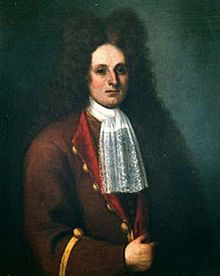
\includegraphics[height=\the\HauteurDesPhotos]{Riccati}&
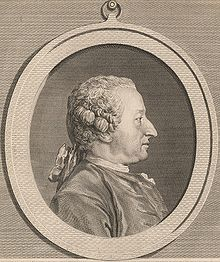
\includegraphics[height=\the\HauteurDesPhotos]{Clairaut}&
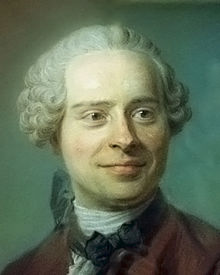
\includegraphics[height=\the\HauteurDesPhotos]{dAlembert}&
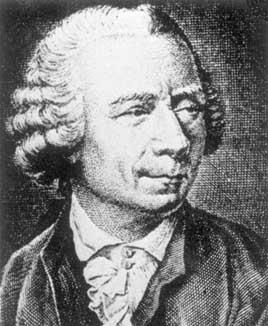
\includegraphics[height=\the\HauteurDesPhotos]{Euler4}\\
Riccati &Clairaut &D'Alembert&Euler%
\end{tabular}}
\bigskip
\ImageADroite{%
On résout les équations différentielles par la méthode des séries entières sans s'encombrer des notions de convergence, bien que l'on entrevoit parfois certaines difficultés dues justement à ces problèmes de convergence... et on en arrive presque aux séries asymptotiques qui ne seront conceptualisées qu'au \textsc{xix}\fup{e} siècle.\\
\indent
Un autre problème reste d'écrire, à l'aide de fonctions simples, les solutions des équations différentielles. La liste des équations différentielles que l'on sait résoudre de cette manière est plutôt maigre:
Leibniz\index[aut]{Leibniz (Gottfried Wilhelm), 1646-1716, Allemand} et sa méthode de décomposition en éléments simples, les Bernouilli et les équations différentielles linéaires du premier ordre, puis Riccati...\index[aut]{Riccati (Jacopo Francesco), 1676-1754, Italien}%
}

\medskip
La découverte par Clairaut\index[aut]{Clairaut (Alexis Claude), 1713-1765, Français} en 1734 de l'existence d'une solution singulière à l'équation~$y - xy' + f(y') = 0$ (à la famille de droites~$y = Cx + f(C)$ qui est l'expression générale des courbes intégrales, il faut adjoindre l'enveloppe de cette famille pour avoir toutes les solutions analytiques de l'équation) relance la dynamique. D'Alembert,\index[aut]{d'Alembert (Jean le Rond), 1717-1783, Français} en 1748, trouve un second cas d'intégrale singulière. Mais c'est Euler\index[aut]{Euler (Leonhard Paul), 1707-1783, Suisse} et Lagrange\index[aut]{Lagrange (Joseph Louis, comte de -), 1736-1813, Italien} qui élucident ce qui se passe en général en exhibant la courbe qui est le lieu des points singuliers.

\medskip
Si l'on sait, dès la fin du \textsc{xvii}\fup{e} siècle intégrer les équations différentielles linéaires du premier et du second ordre à coefficients constants par des sommes d'exponentielles, il faut attendre 1760 pour que la théorie vienne à bout des équations différentielles linéaires à coefficients constants d'ordre quelconque. En 1739, Euler\index[aut]{Euler (Leonhard Paul), 1707-1783, Suisse} rencontre une équation différentielle linéaire à coefficients constants du quatrième ordre sur un problème de vibration des tiges qu'il ne sait pas intégrer. C'est en 1743 qu'il forme ce qu'on appelle aujourd'hui l'équation caractéristique, qu'il complète un peu plus tard lorsqu'une racine de cette équation polynomiale est multiple.

\sbox{\MaBoiteAvecPhotos}{\setlength{\tabcolsep}{0pt}\scriptsize%
\begin{tabular}{cccc}
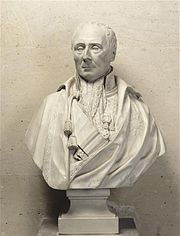
\includegraphics[height=\the\HauteurDesPhotos]{Lagrange2}&
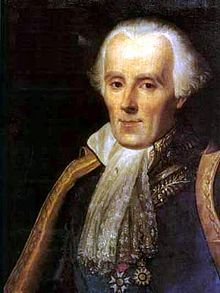
\includegraphics[height=\the\HauteurDesPhotos]{Laplace}&
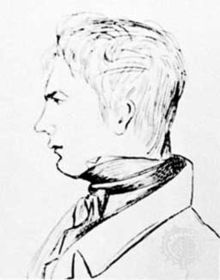
\includegraphics[height=\the\HauteurDesPhotos]{Sturm}&
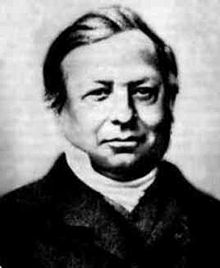
\includegraphics[height=\the\HauteurDesPhotos]{Liouville}\\
Lagrange &Laplace &Sturm&Liouville%
\end{tabular}}
\medskip
\ImageADroite{%
D'Alembert\index[aut]{d'Alembert (Jean le Rond), 1717-1783, Français} remarque que pour les équations différentielles non homogènes, l'adjonction d'une solution particulière à la solution générale de l'équation homogène donne la solution générale de l'équation homogène. Lagrange\index[aut]{Lagrange (Joseph Louis, comte de -), 1736-1813, Italien} introduit la méthode de variation des constantes pour résoudre par quadratures l'équation linéaire non homogène lorsque l'on connaît la solution générale de l'équation homogène.}

\medskip
Clairaut, D'Alembert, Euler, Lagrange et Laplace consacrent de nombreux mémoires au problème des~$n$ corps. Le premier exemple du problème de Sturm-Liouville\index[aut]{Sturm (Jacques Charles François), 1803-1855, Français}\index[aut]{Liouville (Joseph), 1809-1882, Français} est donné par D'Alembert\index[aut]{d'Alembert (Jean le Rond), 1717-1783, Français} à propos de la vibration d'une corde non homogène.
\end{histoire}

\medskip
Les mathématiciens du \textsc{xviii}\fup{e} siècle admettent sans discussion l'existence de solutions des équations différentielles et des équations aux dérivées partielles sans chercher le domaine d'existence de ces solutions. Il faut attendre Cauchy,\index[aut]{Cauchy (Augustin Louis, baron -), 1789-1857, Français} vers 1820, pour que soit abordée l'existence d'une solution à l'équation différentielle~$y' = f(x,y)$, où~$f$ est supposée continument différentiable en chaque variable. Sans connaître les travaux de Cauchy, Lipschitz,\index[aut]{Lipschitz (Rudolph Otto Sigismund), 1832-1903, Allemand} en 1868, retrouve le résultat de Cauchy mais s'affranchit de l'hypothèse de différentiabilité de~$f$ au profit de la condition dite aujourd'hui de Lipschitz. En 1837, Liouville\index[aut]{Liouville (Joseph), 1809-1882, Français} utilise, pour le cas particulier d'une équation linéaire du second ordre une méthode d'approximation successive: on construit une suite de fonctions convergeant vers la solution.
\colorblack


\medskip
Si l'on considère une fonction~$f$, sa dérivée~$f'$ exprime sa variation: positive~$f$ est croissante (et plus sa value est grande, plus la croissance est rapide), négative~$f$ est décroissante...

À partir de là on peut considérer une population de personnes. Le nombre de total de personnes à un instant~$t$ est donné par~$f(t)$. Plus la population est nombreuse, plus elle se reproduit: en d'autres termes, la vitesse de croissance de la population est proportionnelle à la taille de la population. On peut donc écrire:
\begin{equation}
f'(t)=k\,f(t)\end{equation}
C'est une équation différentielle très simple, mais qui modélise le problème dit de dynamique de population.\index{ED-EDP!dynamique de population}

\medskip
Un autre problème simple, toujours en dynamique des populations, est celui de deux populations interdépendantes: les proies~$g(t)$ et le prédateurs~$m(t)$. Les proies se reproduisent et sont mangées par les prédateurs, alors que les prédateurs meurent sauf s'ils peuvent manger des proies.

Cela conduit au système de Lotka-Volterra:\index{ED-EDP!Lotka-Volterra}\index{ED-EDP!système proie-prédateur}\index[aut]{Volterra (Vito), 1860-1940, Italien}\index[aut]{Lotka (Alfred James), 1880-1949, Américain}
\begin{equation}%$\colorgreen
  \begin{cases} g'(t)&=A\,g(t)-B\,g(t)\,m(t) \\ m'(t)&=-C\,m(t)+D\,g(t)\,m(t) \end{cases} 
\end{equation}
où il est nécessaire de résoudre les équations simultanément (on dit que les équations sont couplées).

\medskip
Pour revenir à des exemples plus connus des lecteurs, on n'oubliera pas que la relation fondamentale de la dynamique de Newton: 
\begin{equation} m\ddot{x}=f(x)
\end{equation}
est une d'équation différentielle du second ordre.\index{ED-EDP!relation fondamentale de la dynamique}\index[aut]{Newton (Isaac, Sir -), 1643-1727, Anglais}
On pourrait multiplier les exemples comme l'équation de l'oscillation d'une masse suspendue à un ressort:
\begin{equation}
\ddot{x} = - c \dot{x} - \omega^2x 
\end{equation}%$
avec ($c>0$) ou sans ($c=0$) frottement.

\medskip
Comme on le voit sur les exemples ci-dessus, et comme on s'en souvient sans doute, il est nécessaire, pour déterminer complètement la solution d'une équation différentielle (ou d'une équation aux dérivées partielles), de disposer de valeurs de la solution en certains points. On appelle ces «contraintes», des \textcolorblue{conditions aux limites}.

%Les conditions aux limites types sont présentées au paragraphe suivant.

\medskip
\begin{histoire}%
Concernant les équations aux dérivées partielles, elles sont initialement résolues par des méthodes ad-hoc, le plus souvent géométriques. On n'écrit pas l'équation aux dérivées partielles linéaires. On ne s'étonnera donc pas que la première équation aux dérivées partielles  n'apparaisse qu'assez tard.

\sbox{\MaBoiteAvecPhotos}{\setlength{\tabcolsep}{0pt}\scriptsize%
\begin{tabular}{cccc}
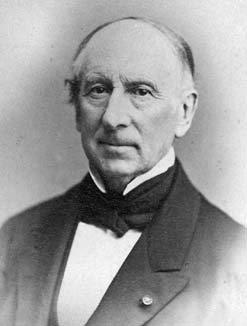
\includegraphics[height=\the\HauteurDesPhotos]{Cauchy3}&
\includegraphics[height=\the\HauteurDesPhotos]{Lipschitz2}&
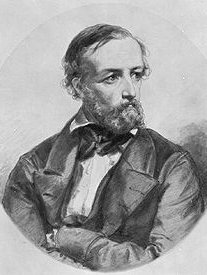
\includegraphics[height=\the\HauteurDesPhotos]{Dirichlet2}&
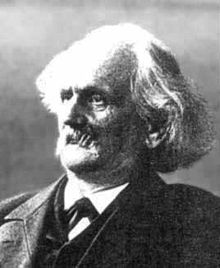
\includegraphics[height=\the\HauteurDesPhotos]{Neumann}\\
Cauchy&Lipschitz&Dirichlet&Neumann%
\end{tabular}}
\medskip
\ImageADroite{%
La théorie de l'intégration des équations aux dérivées partielles du premier ordre ne date que de 1734. L'idée d'Euler\index[aut]{Euler (Leonhard Paul), 1707-1783, Suisse} est de ramener ladite intégration à celle des équations différentielles ordinaires. Euler montre qu'une famille de fonctions dépendant de deux paramètres vérifie une équation aux dérivées partielles du premier ordre en éliminant ces paramètres entre les dérivées partielles. Inversement, une telle équation admet une solution dépendant d'une fonction arbitraire. Il parvient ainsi à intégrer plusieurs équations de ce type.}

\medskip
Lagrange,\index[aut]{Lagrange (Joseph Louis, comte de -), 1736-1813, Italien} dans un mémoire de 1785, résume les connaissances de l'époque sur ces questions. Il ne sait intégrer que onze types d'équations aux dérivées partielles du premier ordre.

\medskip
La solution de l'intégration de ces équations allait venir d'un mathématicien peu connu, mort en 1784, Paul Charpit.\index[aut]{Charpit de Villecourt (Paul), ?-1784, Français} Son mémoire, présenté en 1784 à l'académie des sciences n'a jamais été publié et est resté longtemps une énigme. Une copie de ce mémoire a été trouvée en 1928.
\end{histoire}
\colorblack

\medskip
\section{Conditions aux limites}\index{condition aux limites}
Comme nous venons de le dire, les \textcolorblue{conditions aux limites} sont des contraintes (des valeurs) que l'on impose à la fonction solution (ou à certaines de ces dérivées) sur tout ou partie du domaine~$\Omega$, et/ou sur toute ou partie de sa frontière~$\Gamma=\partial\Omega$.
%%%%%%%%%%%%%%%%%%%%%%
\parvm
D'un point de vue «vocabulaire», certains types de conditions aux limites standard existent qui sont listées ci-après.

\medskip
\subsection{Dirichlet -- valeurs aux bords}\index{condition aux limites!de Dirichlet}\index[aut]{Dirichlet (Johann Peter Gustav Lejeune), 1805-1859, Allemand}
%%%%%%%%%%%%%%%%%%%%%%
\medskipvm
On parle de \textcolorblue{condition de Dirichlet} imposée à une équation différentielle ou une équation aux dérivées partielles, lorsque l'on spécifie les \textcolorred{valeurs} que la solution doit vérifier sur toute ou partie de la frontière du domaine.
%%%%%%%%%%%%%%%%%%%%%%
\medskipvm
Il peut s'agir par exemple d'un déplacement imposé (par exemple nul) en des points d'une structure (points d'appuis rigides).

\medskip
\subsection{Neumann -- gradients aux bords}\index{condition aux limites!de Neumann}\index[aut]{Neumann (Carl Gottfried), 1832-1925, Allemand}

On parle de \textcolorblue{condition de Neumann} imposée à une équation différentielle ou une équation aux dérivées partielles, lorsque l'on spécifie les \textcolorred{valeurs des dérivées} que la solution doit vérifier sur la frontière du domaine (flux, contraintes...)

\medskip
\subsection{Robin -- relation gradient/valeurs sur le bord}\index{condition aux limites!de Robin}\index[aut]{Robin (Victor Gustave), 1855-1897, Français}

On parle de \textcolorblue{condition de Robin} ou \textcolorblue{condition de Fourier} ou \textcolorblue{condition d'impédance} imposée à une équation différentielle ou une équation aux dérivées partielles, lorsque l'on spécifie une \textcolorred{relation linéaire} entre les valeurs de la fonction et les valeurs de la dérivée de la fonction qui est solution du problème sur toute ou partie de la frontière du domaine.
%%%%%%%%%%%%%%%%%%%%%%
\medskipvm
C'est donc une pondération de conditions de Dirichlet et de Neumann.

\medskip
\subsection{Condition aux limites dynamique}\index{condition aux limites!dynamique}
On parle de \textcolorblue{condition aux limites dynamique} imposée à une équation différentielle ou une équation aux dérivées partielles, lorsque l'on spécifie une \textcolorred{combinaison linéaire} entre la dérivée temporelle et la dérivée normale que la solution doit vérifier sur toute ou partie la frontière du domaine.

\medskip
\subsection{Condition aux limites mêlée}\index{condition aux limites!mêlée}
On parle de \textcolorblue{condition aux limites mêlée} lorsque l'on juxtapose plusieurs conditions aux limites différentes sur toute ou partie de la frontière du domaine.

\medskip
\section{Types d'équation aux dérivées partielles}
La forme générale d'une équation aux dérivées partielles linéaire, scalaire, d'ordre 2 est:
\begin{equation}
au + c \nabla u + \dive (A\nabla u) = f
\end{equation}
où~$a: \Omega\rightarrow\RR$, $c: \Omega\rightarrow\RR^n$, 
$A: \Omega\rightarrow\RR^{n\times n}$ et~$f: \Omega\rightarrow\RR$ sont les coefficients de l'équation aux dérivées partielles linéaires.
%%%%%%%%%%%%%%%%%%%%
\medskipvm
Dans le cas où~$u$ est scalaire ($n = 1$) et les coefficients sont constants, on obtient:
\begin{equation}
\alpha\dfrac{\partial^2 u}{\partial x^2}+\beta\dfrac{\partial^2 u}{\partial x\partial y}
+\gamma \dfrac{\partial^2 u}{\partial y^2} + \delta \dfrac{\partial u}{\partial x}
+ \epsilon \dfrac{\partial u}{\partial y} +\gamma u = f
\end{equation}
où~$\alpha$, $\beta$, $\gamma$, $\delta$, $\epsilon$, $\gamma$ sont des scalaires.
Cette équation est dite:
\begin{itemize}
  \item \textcolorblue{elliptique} si~$\beta^2-4\alpha\gamma>0$;
  \item \textcolorblue{parabolique} si~$\beta^2-4\alpha\gamma=0$;
  \item \textcolorblue{hyperbolique} si~$\beta^2-4\alpha\gamma<0$.
\end{itemize}

\medskip
\colorgreen
On peut dire que:
\begin{itemize}
  \item les problèmes elliptiques vont concerner les problèmes stationnaires tels que ceux de la mécanique, la thermique,l'électrostatique, les membranes élastiques,l'écoulement potentiel;
  \item les problèmes paraboliques vont concerner les modèles instationnaires tels que la diffusion thermique (équation de la chaleur), chimique, neutronique, les fluide visqueux incompressible. On parlera d'irréversibilité, de décroissance, de principe du maximum, de propagation à vitesse infinie; 
  \item les problèmes hyperboliques vont concerner les modèles  instationnaires tels que la propagation des ondes, l'électromagnétisme, l'élastodynamique. On parlera de réversibilité, de conservation de l'énergie, de propagation à vitesse finie.
\end{itemize}
\colorblack

\medskip
\section{Phénomènes de propagation et de diffusion}

Dans ce paragraphe, nous avons regroupé les notions de propagation et de diffusion.
\medskipvm
La propagation et la diffusion sont liées. La diffusion, c'est en quelque sorte l'homogénéisation d'une grandeur dans un milieu et dans le temps. Or pour qu'il y ait diffusion, il faut bien que ledit phénomène se propage.

\medskip
Nous nous placerons dans un cadre beaucoup plus macroscopique, où les interactions entre particules sont quantifiées au travers de variables macroscopiques continues, comme par exemple la température, la pression, mais également le frottement fluide, la conductivité thermique, la masse volumique...
\medskipvm
L'analogie de formulation mathématique nous fera également considérer les cas de propagation des ondes dans des milieux donnés. C'est d'ailleurs essentiellement via la propagation des ondes que nous aborderons les formulations... l'équation de la chaleur constituant le liant idéal pour illustrer les liens entre propagation et diffusion.

\medskip
\begin{histoire}%
Le déplacement des atomes, ions ou molécules dans un milieu, que celui-ci soit solide (cristallin ou amorphe), liquide ou gazeux, est appelé de manière générale «migration». 

\sbox{\MaBoiteAvecPhotos}{\setlength{\tabcolsep}{0pt}\scriptsize%
\begin{tabular}{cc}
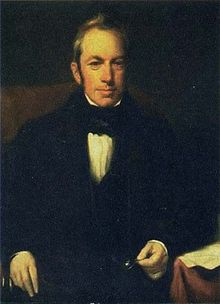
\includegraphics[height=\the\HauteurDesPhotos]{Brown}&
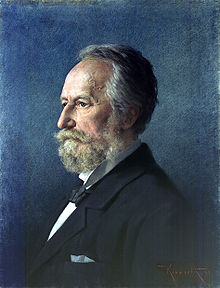
\includegraphics[height=\the\HauteurDesPhotos]{Fick}\\
Brown&Fick%
\end{tabular}}
\medskip
\ImageADroite{%
Au sens large la diffusion désigne des transferts obéissant aux lois de Fick,\index[aut]{Fick (Adolf Eugene), 1829-1901, Allemand} i.e. dont la résultante macroscopique vérifie l'équation de diffusion. La turbulence entraine ainsi une forte diffusion dans les fluides. La diffusion moléculaire est la migration sous l'effet de l'agitation thermique, à l'exception des autres phénomènes. Elle intervient par exemple dans des procédés d'amélioration des caractéristiques mécaniques (traitements de surface comme la nitruration ou cémentation), la résistance à la corrosion et les procédés d'assemblage par brasage.}

\medskip
En 1827, le botaniste Robert Brown\index[aut]{Brown (Robert), 1773-1859, Écossais} observe le mouvement erratique de petites particules de pollen immergées dans de l'eau. Il ne s'agit pas d'un phénomène de diffusion, puisque ce qui bouge est une particule macroscopique, mais cette «marche aléatoire», que l'on appellera «mouvement brownien», servira de modèle pour la diffusion: Le mouvement brownien, ou processus de Wiener, est le mouvement aléatoire d'une «grosse» particule immergée dans un fluide et qui n'est soumise à aucune autre interaction que des chocs avec les «petites» molécules du fluide environnant.  Il en résulte un mouvement très irrégulier de la grosse particule. Ce mouvement, qui permet de décrire avec succès le comportement thermodynamique des gaz (théorie cinétique des gaz), est aussi très utilisé dans des modèles de mathématiques financières.

\medskip
En 1855, Adolph Fick\index[aut]{Fick (Adolf Eugene), 1829-1901, Allemand} propose des lois phénoménologiques, empiriques, inspirées de la loi de Fourier\index[aut]{Fourier (Jean Baptiste Joseph), 1768-1830, Français} pour la chaleur (établie en 1822). C'est Albert Einstein\index[aut]{Einstein (Albert), 1879-1955, Suisse-américain} qui démontrera les lois de Fick\index[aut]{Fick (Adolf Eugene), 1829-1901, Allemand} en 1905 avec ses travaux sur la loi stochastique. La première loi de Fick énonce que «le flux de diffusion est proportionnel au gradient de concentration».
\end{histoire}
\colorblack


\medskip
\subsection{Équations de Laplace et Poisson}
L'\textcolorblue{équation de Laplace, ou Laplacien} est l'équation:\index{ED-EDP!de Laplace}\index[aut]{Laplace (Pierre Simon de -), 1749-1827, Français}\index{laplacien}
\begin{equation}\Delta \varphi=0\end{equation}
Elle est elliptique. 
\medskipvm
Elle apparaît dans de nombreux problèmes physiques: astronomie, électrostatique, mécanique des fluides, propagation de la chaleur, diffusion, mouvement brownien, mécanique quantique.
\medskipvm
Les fonctions solutions de l'équation de Laplace sont appelées les \textcolorblue{fonctions harmoniques}. Toute fonction holomorphe est harmonique.

\medskip
L\textcolorblue{'équation de Poisson} est l'équation:\index{ED-EDP!de Poisson}\index[aut]{Poisson (Siméon Denis), 1781-1840, Français}
\begin{equation}\Delta \varphi=f\end{equation}
où~$f$ est une fonction donnée. Elle est elliptique.
%%%%%%%%%%%%%%%%%%%%%
\medskipvm
Par exemple, en électrostatique, on exprime le potentiel électrique~$V$ associé à une distribution connue de charges~$\rho$ (dans le vide) par la relation:
\begin{equation}
  \Delta V = - \dfrac{\rho}{\epsilon_0}
\end{equation}
En gravitation universelle, le potentiel gravitationnel~$\Phi$ est relié à la masse volumique $\mu$ par la relation:
\begin{equation}
\Delta \Phi = 4 \pi \, G \, \mu 
\end{equation}

\medskip
\subsection{Équation d'onde, phénomènes vibratoires}\label{Sec-EqOnde}
Il s'agit encore d'une extension de l'équation de Laplace.
\medskipvm
L'\textcolorblue{équation d'onde} est l'équation générale qui décrit la propagation d'une onde (sonore ou électromagnétique dont la lumière), qui peut être représentée par une grandeur scalaire ou vectorielle.
\medskipvm
Dans le cas vectoriel, en espace libre, dans un milieu homogène, linéaire et isotrope, l'équation d'onde s'écrit:\index{ED-EDP!des ondes}
\begin{equation}
  \Delta u = - \frac1{c^2} \dfrac{\partial^2 u}{\partial t^2} \quad \text{ ou } \quad \square u =0
\end{equation}
où la fonction d'onde inconnue est notée~$u(x,y,z,t)$, $t$ représente le temps, et le nombre~$c$ représente la célérité ou vitesse de propagation de l'onde~$u$ (rappel:~$\square$ est le d'Alembertien). Elle est hyperbolique.

\medskip
Dans le cas de \textcolorblue{l'acoustique}, alors cette équation est obtenue à partir des équations de la mécanique ainsi que de l'hypothèse de fluide parfait:
\begin{itemize}
  \item conservation de la masse:~$\dot{\rho}+\dive(\rho u)=0$ avec 
	$\rho$ la masse volumique du milieux et~$u$ sa vitesse;
  \item conservation de la quantité de mouvement:~$\dive(\sigma)=\rho\dot{u}$, avec
	$\sigma$ le tenseur des contraintes
  \item le fluide est parfait, et sa relation de comportement est donc:~$\sigma=-p'I$ avec
	$p'$ la pression dans le fluide.
\end{itemize}
\medskipvm
À partir de ces trois équations, on retrouve l'équation des ondes sous la forme:\index{ED-EDP!de l'acoustique}
\begin{equation}\label{Eq-EqOndeAcou}
\Delta p' - \dfrac1{c^2} \ddot{p}' = 0
\end{equation}
avec~$c$ la célérité de l'onde acoustique dans le milieu (vitesse du son).

\medskip
L'équation des ondes permet également de modéliser le problème de l'évolution de la déformation d'une membrane tendue (peau de tambour).\index{ED-EDP!de la déformation d'une membrane} Dans ce cas là, on note plutôt:
\begin{equation}
 \sigma \Delta u = \rho\ddot{u} \text{ dans }\Omega
\end{equation}
où~$\Omega$ est notre domaine qui est une surface, donc~$\Omega\subset\RR^2$.

\textcolorblue{La même équation en dimension deux ou trois modélise la plupart des phénomènes vibratoires.} En dimension 1, cette équation s'appelle l'\textcolorblue{équation des cordes vibrantes.}


\medskip
\subsection{Équation de la chaleur}

L'\textcolorblue{équation de la chaleur} est une équation aux dérivées partielles parabolique, introduite au début du \textsc{xix}\fup{e} siècle par Fourier pour décrire le phénomène physique de conduction thermique.\index{ED-EDP!de la chaleur}\index[aut]{Fourier (Jean Baptiste Joseph), 1768-1830, Français}

\medskip
\begin{histoire}%
En dépit des railleries de Hugo\index[aut]{Hugo (Victor), 1802-1885, Français} et Stendhal\index[aut]{Beyle (Henri), dit Stendhal, 1783-1842, Français} à son encontre, Joseph Fourier\index[aut]{Fourier (Jean Baptiste Joseph), 1768-1830, Français} laissera son nom à la postérité à plus d'un titre:\\[-2.5mm]
\sbox{\MaBoiteAvecPhotos}{\setlength{\tabcolsep}{0pt}\scriptsize%
\begin{tabular}{cc}
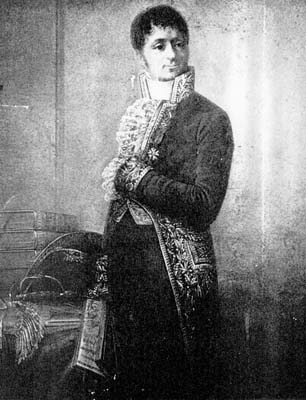
\includegraphics[height=\the\HauteurDesPhotos]{Fourier2}&
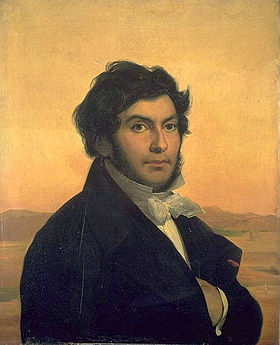
\includegraphics[height=\the\HauteurDesPhotos]{Champollion}\\
Fourier&Champollion%
\end{tabular}}
\ImageADroite{%
\noindent en tant qu'égyptologue, une spécialité  qu'il bouleverse à la suite de sa participation à l'expédition napoléonienne de 1798 (en 1810, il créera l'Université Royale de Grenoble, dont il deviendra le recteur, et y remarquera Jean-François Champollion.\index[aut]{Champollion (Jean-François), 1790-1832, Français} Ils sont enterrés au cimetière du Père-Lachaise à côté l'un de l'autre); en tant qu'homme politique puisqu'il est préfet d'Isère sous Napoléon Bonaparte\index[aut]{Bonaparte (Napoléon), 1769-1821, Français} et sous la Restauration; en tant qu'administrateur, comme réorganisateur des statistiques françaises; et enfin en tant que scientifique, la consécration de sa carrière étant son élection au poste de secrétaire perpétuel de l'Académie des Sciences. Pour tous les mathématiciens, il reste le fondateur de l'analyse de Fourier, qu'il crée au début du \textsc{xix}\fup{e} siècle pour étudier mathématiquement la répartition de chaleur dans un corps conducteur.}

Quelques repères chronologiques:
En 1807, Fourier écrit l'équation de la chaleur.
En 1808, son mémoire est accepté par l'Académie des Sciences en dépit de sérieuses critiques concernant la rigueur des démonstrations (Fourier a en particulier une controverse avec Poisson).\index[aut]{Poisson (Siméon Denis), 1781-1840, Français}
En 1822 a lieu la publication du \emph{Traité analytique de la chaleur}, version remaniée et augmentée de son mémoire, qui s'imposera comme l'un des ouvrages scientifiques majeurs du dix-neuvième siècle.

\medskip
La lecture du \emph{Traité analytique} est toujours profitable. La première phrase sonne comme une profession de foi: «Les causes primordiales ne nous sont point connues; mais elles sont assujetties à des lois simples et constantes, que l'on peut découvrir par l'observation, et dont l'étude est l'objet de la philosophie naturelle». Fourier\index[aut]{Fourier (Jean Baptiste Joseph), 1768-1830, Français} confesse donc son ambition de décrire des phénomènes physiques jusque là jugés inaccessibles, par le moyen des mathématiques; il le confirme dans le choix d'une devise en latin (attribuée par Fourier à Aristote,\index[aut]{Aristote (dit le Stagirite), -384-- -322, Grec} mais probablement inventée par lui-même) : \emph{Et ignem regunt numeri} (Même le feu est régi par les nombres).

\medskip
L'idée maîtresse de Fourier,\index[aut]{Fourier (Jean Baptiste Joseph), 1768-1830, Français} celle que l'on lui attribue le plus naturellement, consiste à décomposer une fonction périodique arbitraire sous forme de série trigonométrique déjà mentionnée à l'équation~(\ref{Eq-FourierTrigo}). Des décompositions de ce style ne sont pas à proprement parler nouvelles: elles faisaient partie du répertoire des analystes de la fin du \textsc{xviii}\fup{e} siècle, à commencer par le plus impressionnant d'entre eux, le Suisse Euler.\index[aut]{Euler (Leonhard Paul), 1707-1783, Suisse} Mais Fourier est le premier à avoir l'intuition du caractère universel et particulièrement commode de cette décomposition trigonométrique.

Fourier donne quelques exemples frappants pour montrer que «n'importe quelle» fonction est décomposable en série trigonométrique: une fonction «en dents de scie» et une autre «en créneaux». Ainsi, même des fonctions discontinues peuvent être exprimées en séries de Fourier, pourvu que l'on définisse la fonction aux points de discontinuité en utilisant la «condition de demi-somme»:
\begin{equation}\label{Eq-Demi-Somme}
f(x)=\dfrac{f(x^+)+f(x^-)}2
\end{equation}

\sbox{\MaBoiteAvecPhotos}{\setlength{\tabcolsep}{0pt}\scriptsize%
\begin{tabular}{c}
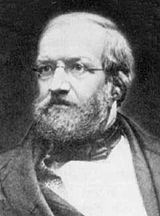
\includegraphics[height=\the\HauteurDesPhotos]{Dirichlet3}\\
Dirichlet%
\end{tabular}}
%\medskip
\ImageAGauche{%
Cela pouvait paraître surprenant à l'époque de Fourier, mais bien sûr ce n'est pas contradictoire avec les théorèmes connus: une série de fonctions continues n'est pas en général continue.
L'acte de foi suivant consiste à admettre que des décompositions similaires s'appliquent à des fonctions non périodiques (définies sur~$\RR$ tout entier). Dans tous les cas, la formule donnant les coefficients de Fourier~(\ref{Eq-FourierAk}) conduit immédiatement à quelques questions, et notamment: comment trouver les coefficients? (problème de l'analyse) En quel sens faut-il comprendre la convergence de ces séries?\\
\indent
La convergence des séries de Fourier est reconnue dès le début comme un problème important et délicat, sur lequel Fourier lui-même avait été attaqué. Le résultat qui fait référence en la matière est le théorème de Dirichlet (1829):\index[aut]{Dirichlet (Johann Peter Gustav Lejeune), 1805-1859, Allemand}}
\begin{theoreme}[Théorème de Dirichlet]\index{théorème!de Dirichlet}
Soit $f: \TT\rightarrow\CC$, continue par morceaux, satisfaisant la condition de demi-somme~(\ref{Eq-Demi-Somme}) et $C^1$ de part et d'autre de chaque point de discontinuité, alors:
\begin{equation}
\forall x\in\TT, \qquad \dsum_{k\in\ZZ} c_k(f)e^{2i\pi kx} = f(x)
\end{equation}
\end{theoreme}

\sbox{\MaBoiteAvecPhotos}{\setlength{\tabcolsep}{0pt}\scriptsize%
\begin{tabular}{cc}
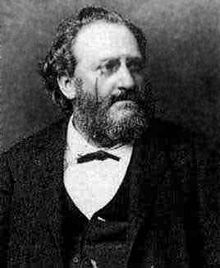
\includegraphics[height=\the\HauteurDesPhotos]{duBois-Reymond}&
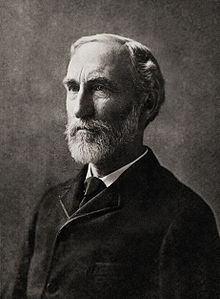
\includegraphics[height=\the\HauteurDesPhotos]{Gibbs}\\
du Bois-Reymond&Gibbs%
\end{tabular}}
\medskip
\ImageADroite{%
Jusqu'en 1873 les spécialistes pensaient que l'hypothèse de continuité $C^1$ de part et d'autre était superflue; mais dans son article \emph{Eine neue Theorie der Convergenz und Divergenz von Reihen mit positiven Gliedern}, du Bois-Reymond,\index[aut]{du Bois-Reymond (Paul David Gustave), 1831-1889, Allemand} donna un contre-exemple sous la forme d'une fonction continue périodique dont la série de Fourier diverge en un point. Si l'on veut avoir la propriété de reconstruction ponctuelle, on doit supposer une certaine régularité; tout au mieux on peut relaxer l'hypothèse~$C^1$.\\
\indent
Même quand elle est vraie, la convergence ponctuelle des séries de Fourier peut être médiocre. Un exemple bien connu est le phénomène de Gibbs,\index[aut]{Gibbs (Josiah Willard), 1839-1903, Américain} qui pose des problèmes pratiques: la série de Fourier d'une fonction créneau présente des oscillations près des points de discontinuité, dont l'ampleur ne s'atténue pas quand le nombre de fréquences tend vers l'infini.}
\end{histoire}
\colorblack

\medskip
Soit~$\Omega$ un domaine de~$\RR^3$ de frontière~$\Gamma=\partial \Omega$ et~$T(x,t)$ un champ de température sur ce domaine (champ de scalaires). 
En présence d'une source thermique dans le domaine, et en l'absence de convection, i.e. de transport de chaleur (i.e. on s'intéresse à la propagation de la température au sein d'un milieu «stable», \textcolorgreen{i.e. qui ne bouge pas; on ne s'intéresse pas à la propagation de chaleur due par exemple à l'existence d'un courant d'air, d'un courant de convection. La convection est plutôt un problème de mécanique des fluides.)}, l'équation de la chaleur s'écrit:
\begin{equation}
\forall x \in\Omega, \quad \frac{\partial T (x,t)}{\partial t} = D \, \Delta T(x,t) + \frac{f}{\rho c}
\end{equation}
où:
\begin{itemize}
  \item~$\Delta$ est l'opérateur Laplacien;
  \item~$D$ est le coefficient de diffusivité thermique (en~$m^2/s$);
  \item~$f$ une éventuelle production volumique de chaleur (en~$W/m^3$);
  \item~$\rho$ est la masse volumique du matériau (en~$kg/m^3$);
  \item~$c$ la chaleur spécifique massique du matériau (en~$J/kg·K$).
\end{itemize}
\medskipvm\colorgris
L'équation de la chaleur est donc une équation de la forme:
\begin{equation}
\dot{u}-\Delta u=f
\end{equation}
Elle est parabolique.\colorblack
%%%%%%%%%%%%%%%%%%%%%
\medskipvm
Pour que le problème soit bien posé, il faut spécifier:
\begin{itemize}
  \item une condition initiale:
  \begin{equation}\forall x\in\Omega, \quad T (x,0) = T_0(x)\end{equation}
  \item une condition aux limites sur le bord du domaine, par exemple:
  \begin{itemize}
  \item de Dirichlet:\begin{equation}\forall x\in\partial \Omega, \quad T (x,t) = 0\end{equation}
  \item de Neumann:\begin{equation}\forall x\in\partial \Omega, \quad \frac{\partial T (x,t)}{\partial n} = n(x) \cdot \nabla T(x,t) = 0\end{equation} où~$n(x)$ est le vecteur normal unitaire au point~$x$.
	\end{itemize}
\end{itemize}
%%%%%%%%%%%%%%%%%%%%%
\medskipvm
L'équation de la chaleur, introduite initialement pour décrire la conduction thermique, permet de décrire le phénomène de diffusion.

La diffusion est un phénomène de transport irréversible qui se traduit à terme par une homogénéisation de la grandeur considérée (par exemple la température dans un domaine, la concentration en produits chimiques dans une solution...).

D'un point de vue phénoménologique, et au premier ordre, ce phénomène est régi par une \textcolorblue{loi de Fick} (par exemple sorption d'eau dans les matériaux composites, diffusion d'actifs au travers de la peau).\index[aut]{Fick (Adolf Eugene), 1829-1901, Allemand} Dans l'équation précédente, $T$ représente alors la répartition de la grandeur considérée (eau dans un composite, concentration d'un constituant chimique...) et le terme source dans~$\Omega$ est souvent nul (i.e.~$f=0$).

\begin{histoire}%
\textbf{À propos de l'effet régularisant de la chaleur:}

L'équation de la chaleur a un «effet régularisant»: quelque soit la distribution initiale de la température pour un problème donné, même discontinue, on aboutit rapidement à une distribution continue et même lisse de la température.

\sbox{\MaBoiteAvecPhotos}{\setlength{\tabcolsep}{0pt}\scriptsize%
\begin{tabular}{ccc}
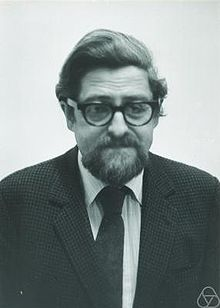
\includegraphics[height=\the\HauteurDesPhotos]{Nirenberg}&
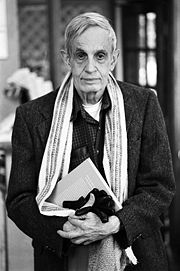
\includegraphics[height=\the\HauteurDesPhotos]{Nash}&
\includegraphics[height=\the\HauteurDesPhotos]{DeGiorgi}\\
Nirenberg&Nash&De Giorgi%
\end{tabular}}
\medskip
\ImageADroite{%
En 1956, Louis Nirenberg\index[aut]{Nirenberg (Louis), 1925- , Américain} propose un nouveau problème à John Nash\index[aut]{Nash (John Forbes), 1928- , Américain} (qui est «aussi pressé que X, aussi exaspérant que Y, quels que soient X et Y» selon Warren Ambrose): la continuité des solutions de l'équation de la chaleur dans les milieux discontinus, i.e. lorsque le coefficient de conductivité est quelconque, et peut même varier brutalement d'un point à l'autre et que l'on a seulement des bornes inférieure et supérieure sur la conductivité.\\ \indent
John Nash\index[aut]{Nash (John Forbes), 1928- , Américain} résout le problème, notamment à l'aide du concept d'entropie de Boltzmann,\index[aut]{Boltzmann (Ludwig), 1944-1906, Autrichien} mais n'obtiendra pas le triomphe escompté, le problème ayant été résolu, en même temps, mais par une autre méthode, par l'italien De Giorgi,\index[aut]{De Giorgi (Ennio), 1928-1996, Italien} qui lui deviendra célèbre.}
Mais John Nash\index[aut]{Nash (John Forbes), 1928- , Américain} est célèbre pour bien d'autres travaux... dont l'un d'eux lui a valu le prix Nobel d'économie en 1994. On pourra regarder le film «un homme d'exception» (\emph{A Beautiful Mind}) de Ron Howard\index[aut]{Howard (Ronald William), 1954- , Américain} en 2001 sur John Nash.
\end{histoire}
\colorblack



\medskip
\section{Mécanique des fluides}
La mécanique des fluides est l'une des deux composantes de la mécanique des milieux continus; l'autre composante étant la mécanique des solides qui sera traitée un peu plus loin.





\medskip
\subsection{Équation de Navier-Stokes}\label{Sec-NavierStokes}
Les équations de Navier-Stokes sont des équations aux dérivées partielles non linéaires qui décrivent le mouvement des fluides newtoniens (visqueux) dans l'approximation des milieux continus. Elles modélisent par exemple les mouvements de l'air de l'atmosphère, les courants océaniques, l'écoulement de l'eau dans un tuyau, et de nombreux autres phénomènes d'écoulement de fluides.

\medskip
Nous considérons l'équation de Navier-Stokes sous la forme:\index{ED-EDP!de Navier-Stokes}\index[aut]{Navier (Claude Louis Marie Henri), 1785-1836, Français}\index[aut]{Stokes (George Gabriel), 1819-1903, Anglais}
\begin{equation}
\rho \dot{u} + \rho (u\cdot\nabla)u - \eta \Delta u
- \left( \zeta + \frac{\eta}{3} \right) \gradb (\dive u)
= \rho f - \nabla p
\end{equation}
où:
\begin{itemize}
  \item~$u$ est la vitesse du fluide ;
  \item~$p$ est la pression dans le fluide ;
  \item~$\rho$ est la masse volumique du fluide;
  \item~$\eta$ est la viscosité dynamique en cisaillement du fluide;
  \item~$\zeta$ est la viscosité dynamique en compression du fluide;
  \item~$f$ est une force massique s'exerçant dans le fluide (par exemple: pesanteur).
\end{itemize}

\medskip
Si de plus le fluide est incompressible (bonne approximation pour les liquides), alors~$\dive u = 0$ 
et l'équation se simplifie:
\begin{equation}
\rho \dot{u} + \rho (u\cdot\nabla)u - \eta \Delta u
= \rho f - \nabla p
\end{equation}
\begin{histoire}%
Des 23 problèmes de Hilbert\index[aut]{Hilbert (David), 1862-1943, Allemand} énoncés en 1900, la moitié est aujourd'hui complètement résolue, l'un a été démontré indécidable, cinq ne le sont pas du tout, les autres étant partiellement traités.

\sbox{\MaBoiteAvecPhotos}{\setlength{\tabcolsep}{0pt}\scriptsize%
\begin{tabular}{cccc}
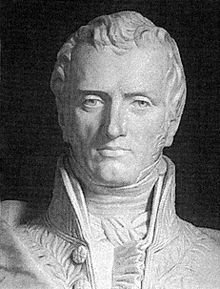
\includegraphics[height=\the\HauteurDesPhotos]{Navier}&
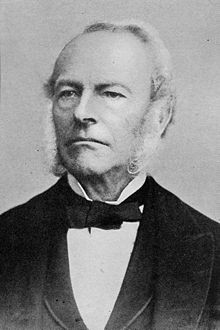
\includegraphics[height=\the\HauteurDesPhotos]{Stokes}&
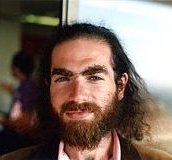
\includegraphics[height=\the\HauteurDesPhotos]{Perelman}&
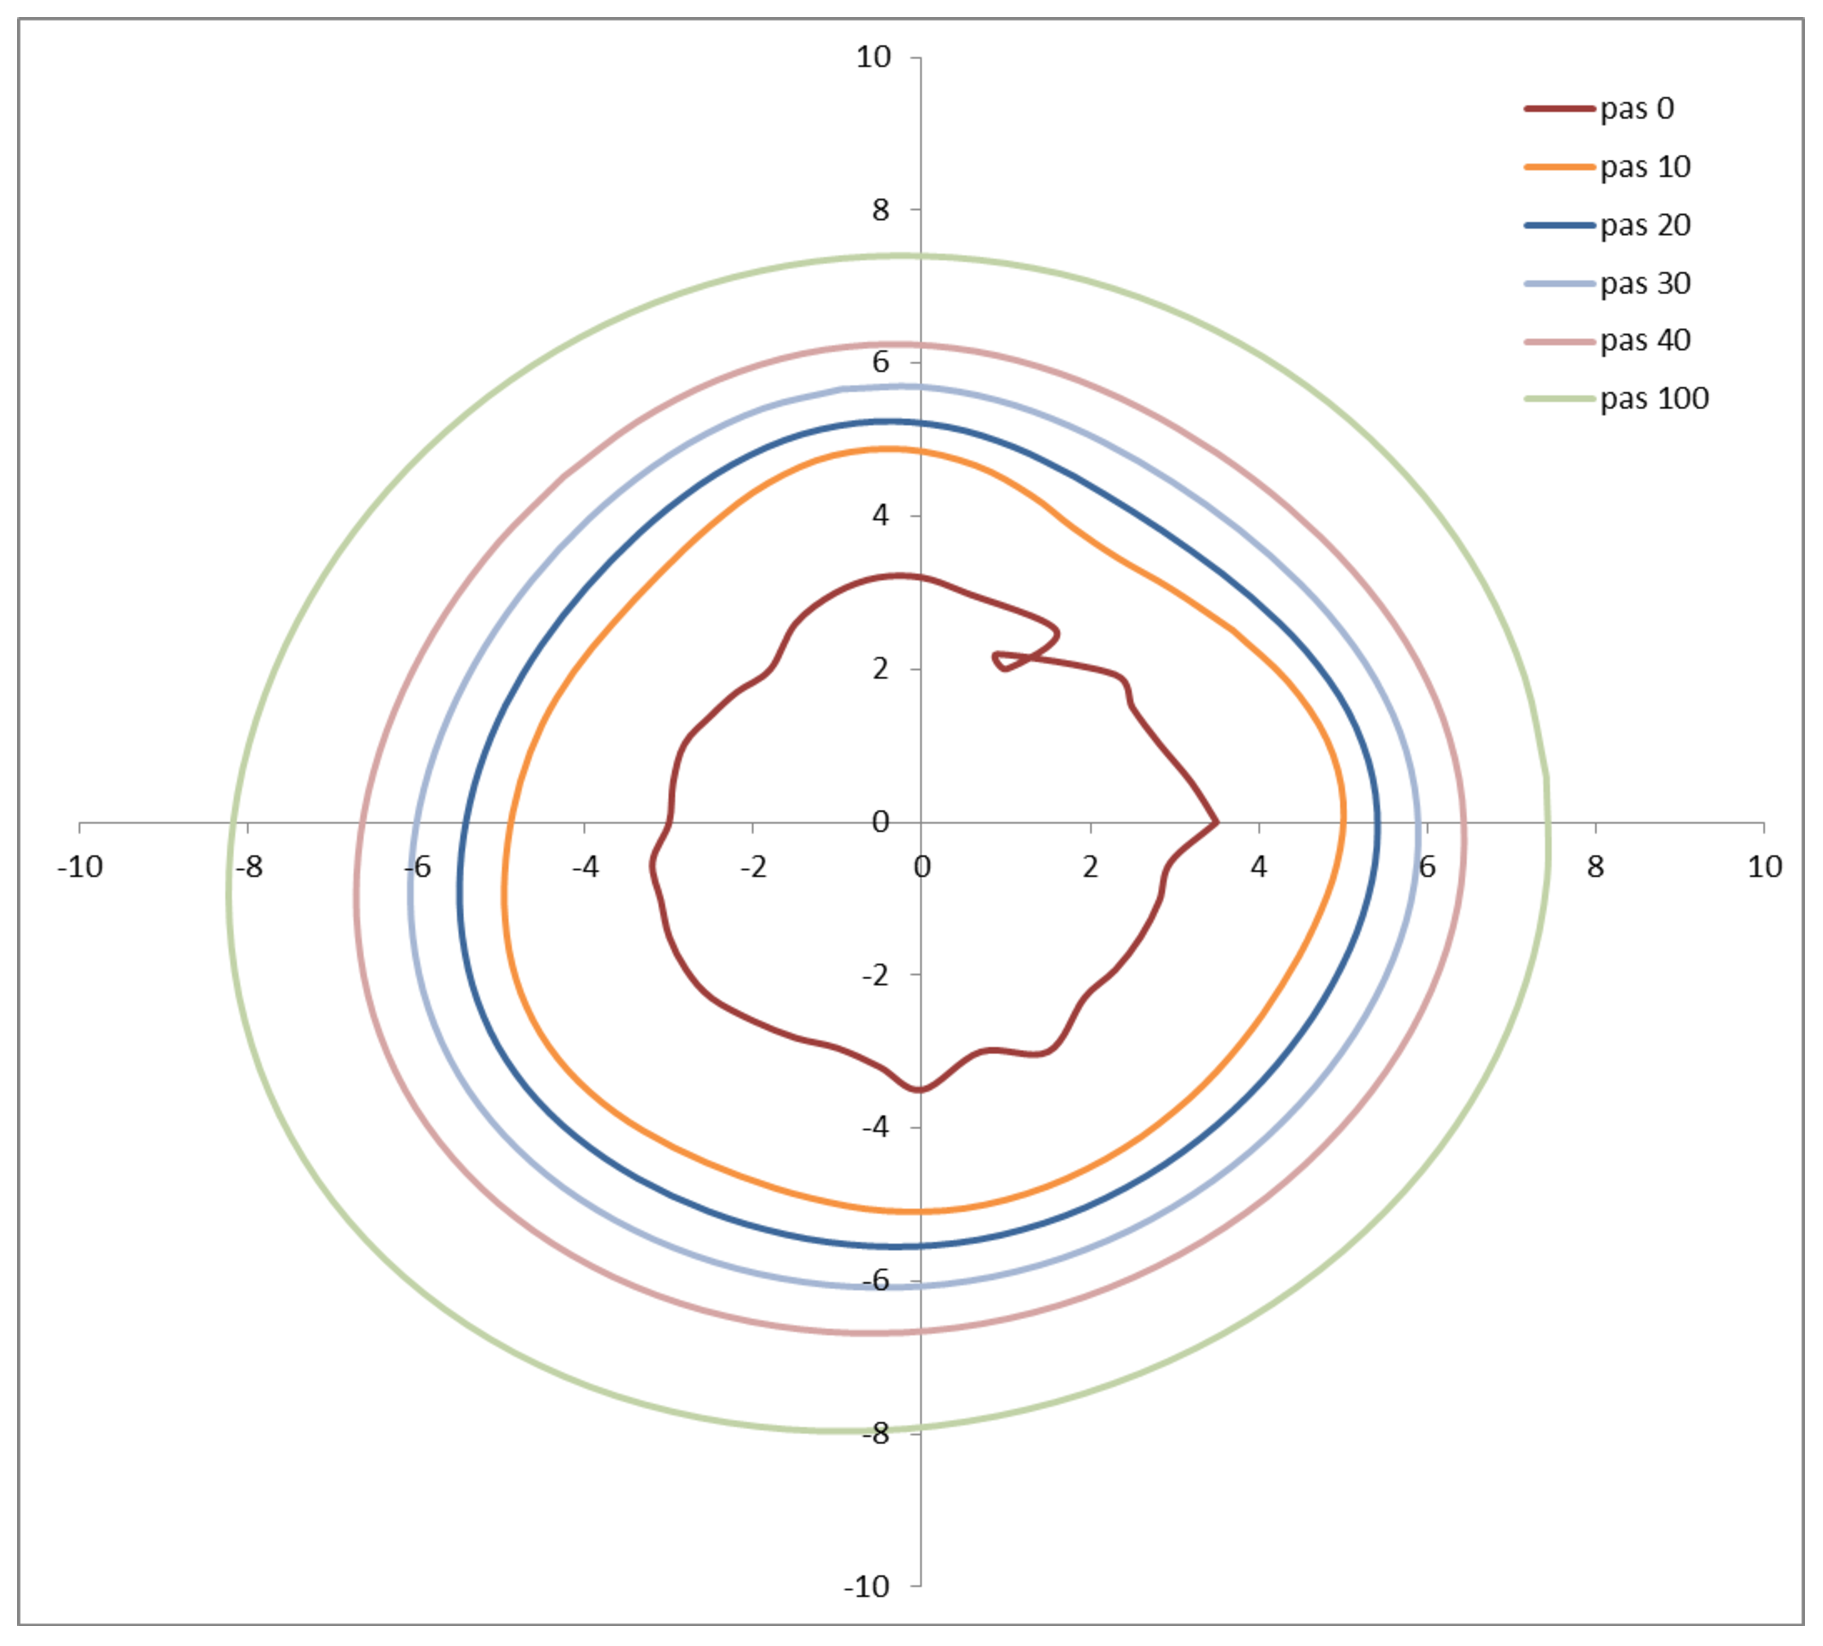
\includegraphics[height=\the\HauteurDesPhotos]{Ricci}\\
Navier &Stokes &Perelman&Ricci%
\end{tabular}}

\medskip
\ImageADroite{%
Des sept problèmes de l'institut Clay (ou problèmes du prix du millénaire, dotés chacun d'un million de dollars américains) énoncés en 2000, seule la conjecture de Poincaré\index[aut]{Poincaré (Henri), 1854-1912, Français} a été démontrée en 2003 par Grigori Perelman\index[aut]{Perelman (Grigori Iakovlevitch), 1966- , Russe} (qui a refusé le prix, ainsi que la médaille Field. D'ailleurs il n'a pas publié son travail dans un journal, mais l'a rendu publique et gratuit sur internet...). Notons au passage que Grigori Perelman\index[aut]{Perelman (Grigori Iakovlevitch), 1966- , Russe} est analyste, i.e. un spécialiste des équations aux dérivées partielles, un sujet que beaucoup de topologues avaient l'habitude de regarder de loin. Ils ont changé d'avis depuis!}

\sbox{\MaBoiteAvecPhotos}{\setlength{\tabcolsep}{0pt}\scriptsize%
\begin{tabular}{c}%
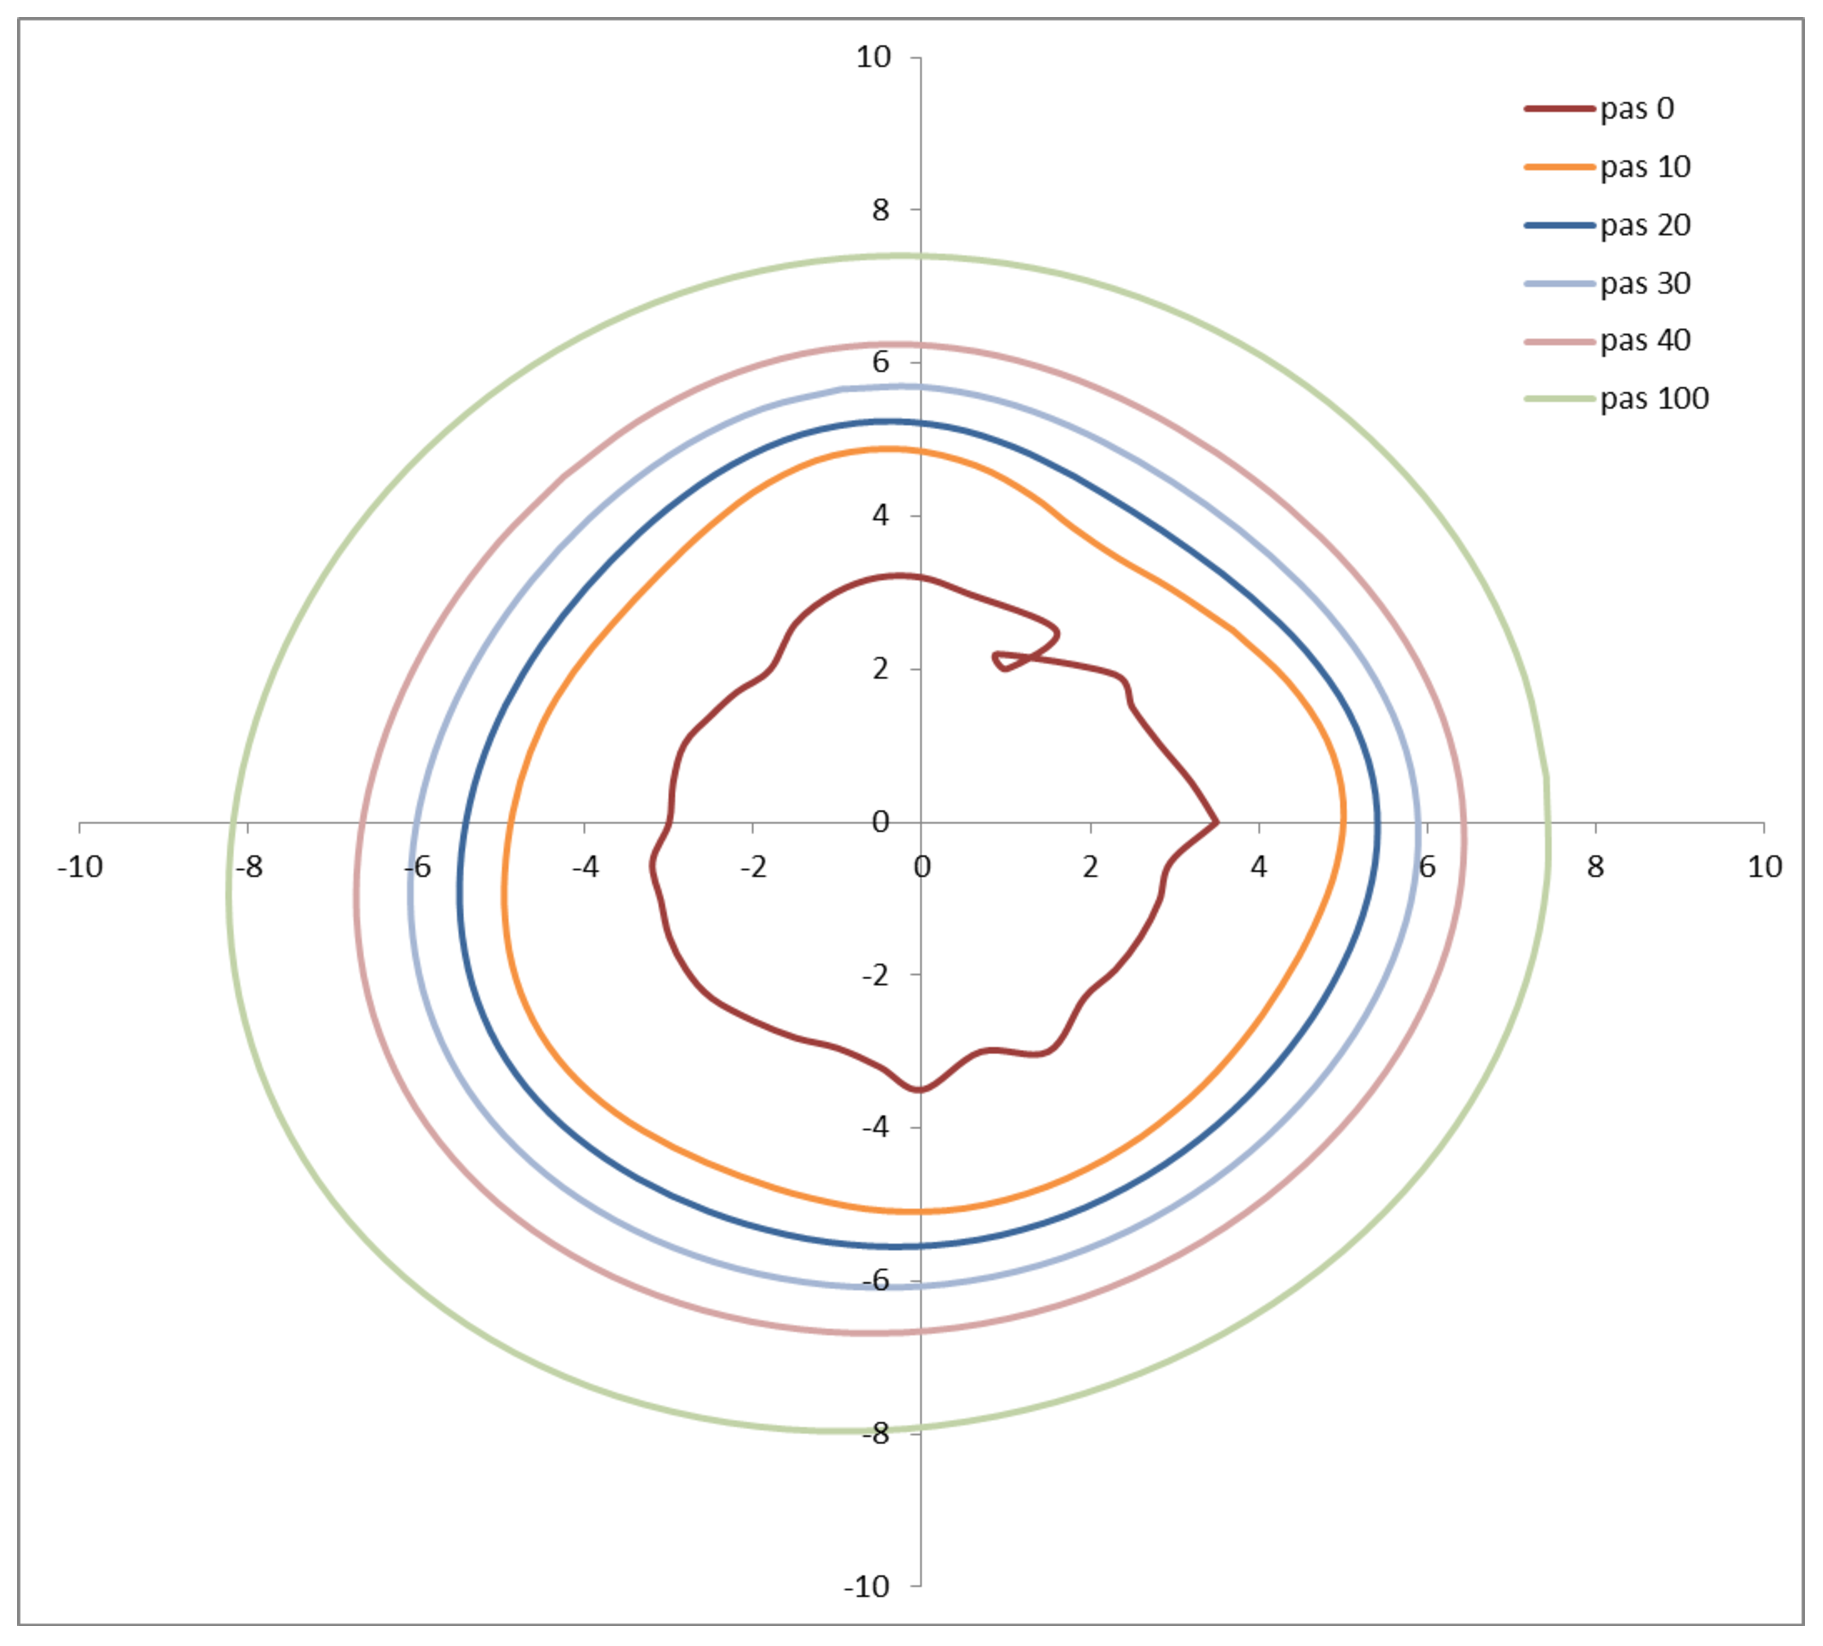
\includegraphics[height=40mm]{Ricci.eps}%
\end{tabular}}
\medskip
\ImageAGauche{%
Pour information, la preuve de Perelman suit le programme de Hamilton,\index[aut]{Hamilton (Richard Streit), 1943-, Américain} qui le premier a pensé à utiliser le flot de Ricci\index[aut]{Ricci-Curbastro (Gregorio), 1853-1925, Italien} pour s'attaquer à ce problème.
Deux mots en aparté sur le flot de Ricci dont on entend beaucoup parlé en ce moment...\\ \indent 
Regardons se qui se passe dans le plan. On part d'une courbe (au centre de l'image ci-contre) qui est «biscornue» et peut même comporter des boucles. Si on la modifie de sorte que chacun de ses points est bougé proportionnellement à sa courbure, alors on obtient une seconde courbe, un peu plus lisse... et en itérant le procédé, on finit par retomber sur un cercle (i.e. sur une sphère en dimension 2), et donc on «voit» que la conjecture de Poincaré\index[aut]{Poincaré (Henri), 1854-1912, Français} est vraie. En d'autres termes, le flot de Ricci permet d'homogénéiser la courbure de la courbe (de la variété dans le cas général).}

\medskip
Le problème des équations de Navier-Stokes\index[aut]{Navier (Claude Louis Marie Henri), 1785-1836, Français}\index[aut]{Stokes (George Gabriel), 1819-1903, Anglais}  figure parmi ces sept problèmes, c'est dire si le problème n'est pas simple. Et c'est, des sept problèmes du millénaire, le seul qui soit en lien direct avec la physique (en lien très direct...). De plus, l'Institut Clay n'a pas fixé comme objectif la démonstration de l'existence de solutions pour les équations de Navier-Stokes et la démonstration que les solutions, si elles existent, sont uniques. Il a «simplement» proposé de récompenser des «progrès essentiels» sur le sujet. Pourtant des calculs en mécaniques des fluides sont effectués chaque jour, par exemple au sein de bureaux d'études pour dimensionner des voitures en aérodynamique.

On n'a pas pu prouver, pour ces équations, qu'il existe en toutes circonstances une solution parfaitement déterminée par les conditions initiales. Pour expliquer sommairement où réside la difficulté avec ces équations, on pourrait dire qu'avec les équations de Navier-Stokes, on passe du discret au continu.

\medskip
Le problème c'est que l'on n'est pas sûr que ce qui est calculé est réellement une solution approchée et si le résultat est fidèle à la réalité: nous nous trouvons dans un cas où l'existence et l'unicité des solutions n'est pas facile à prouver. S'il existe des cas où des solutions régulières sont parfaitement déterminées à partir des conditions aux limites, cela n'est pas vrai en toutes circonstances et pour tous temps (on ne sait pas si une solution régulière ne peut pas devenir turbulente près un temps suffisamment long par exemple).

\sbox{\MaBoiteAvecPhotos}{\setlength{\tabcolsep}{0pt}\scriptsize%
\begin{tabular}{cccc}
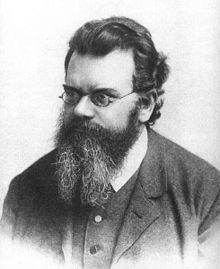
\includegraphics[height=\the\HauteurDesPhotos]{Boltzmann}&
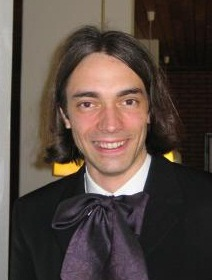
\includegraphics[height=\the\HauteurDesPhotos]{Villani}&
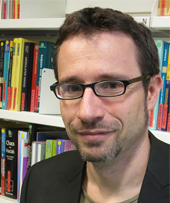
\includegraphics[height=\the\HauteurDesPhotos]{Desvillettes}&
\includegraphics[height=\the\HauteurDesPhotos]{Toscani}\\
Boltzmann&Villani&Desvillettes&Toscani%
\end{tabular}}
\medskip
\ImageADroite{%
La non linéarité de ces équations joue des tours conduisant à des solutions qui peuvent par exemple ne pas se superposer sans s'influencer (alors que ce n'est pas le cas avec les équations linéaires). La viscosité n'est pas exempte de problème non plus, puisqu'elle conduit aux turbulences (que l'on pourrait qualifier de problème de passage d'échelle).  D'ailleurs une description à un niveau intermédiaire entre une description atomiste (microscopique) et une description continue (macroscopique) a été faite par Boltzmann\index[aut]{Boltzmann (Ludwig), 1944-1906, Autrichien} (niveau mésoscopique, description statistique), mais nous ne la présenterons pas ici.
Les travaux de Cédric Villani\index[aut]{Villani (Cédric), 1973- , Français} (médaillé Fields 2010) ont répondu en grande partie au problème de la théorie cinétique (qui décrit un système constitué d'un très grand nombre de particules en interaction). Il a également prouvé des formes quantifiées du second principe de la thermodynamique: Boltzmann avait prouvé la croissance de l'entropie, et Cédric Villani en collaboration avec Laurent Desvillettes\index[aut]{Desvillettes (Laurent), 1966- , Français} et Giuseppe Toscani\index[aut]{Toscani (Giuseppe), ?- , Italien} a permis de quantifier la production d'entropie et le retour à l'équilibre. Ses travaux sur l'effet Landau\index[aut]{Landau (Lev Davidovitch), 1908-1968, Russe} (phénomène de relaxation non collisionnelle) ont des répercussions théoriques et pratiques, par exemple dans les modèles de mécanique classique en astrophysique.}

\medskip
La description faible du problème, qui sera présentée dans un autre chapitre, comporte elle-aussi ses problèmes car on n'est pas sûr de la convergence vers la solution forte.

Bien que des résultats d'existences et d'unicité existent, aucun ne permet soit de conclure à l'existence de solutions régulières pour tout temps, soit à l'apparition de singularité... On retrouve ici la notion de chaos, déterministe ou non, que nous n'aborderons pas dans ce document, mais pour lequel il est aisé de trouver de la documentation. Signalons quand même qu'il est identique de parler de dynamique non linéaire ou de théorie du chaos. On pourra donc se servir de ces deux points d'entrée pour toute recherche sur le sujet.
\end{histoire}
\colorblack


\medskip
\subsection{Équation de Stokes}

Il s'agit d'un cas particulier de l'équation de Navier-Stokes (termes inertiels absents ou négligés).

Lorsqu'un fluide visqueux s'écoule lentement en un lieu étroit ou autour d'un petit objet, les effets visqueux dominent sur les effets inertiels. Son écoulement est alors appelé écoulement de Stokes. On parle aussi d'écoulement à faible nombre de Reynolds (le nombre de Reynolds\index[aut]{Reynolds (Osborne), 1842-1912, Irlandais} mesure le poids relatif des termes visqueux et inertiel dans l'équation de Navier-Stokes). Ce nombre de Reynolds est alors beaucoup plus petit que~$1$.

\medskip
L'équation de Stokes, qui décrit l'écoulement d'un fluide newtonien incompressible en régime permanent et à faible nombre de Reynolds,\index[aut]{Reynolds (Osborne), 1842-1912, Irlandais} s'écrit dans~$\Omega$:\index{ED-EDP!de Stokes}\index[aut]{Stokes (George Gabriel), 1819-1903, Anglais}
\begin{equation}
-\eta \Delta u + \nabla p = \rho f
\end{equation}

On rappelle que si de plus le fluide est incompressible, alors on a également 
$\dive u = 0$ dans~$\Omega$.


\medskip
Contrairement à l'équation de Navier-Stokes, l'équation de Stokes est linéaire. Les écoulements solutions de cette équation possèdent par conséquent des propriétés bien particulières:
\begin{description}
  \item[\textcolorblue{unicité:}]
	pour des conditions aux limites données (valeur de la vitesse au niveau des parois et/ou à l'infini), il existe un et un seul écoulement vérifiant l'équation de Stokes;
  \item[\textcolorblue{additivité:}] 
	les solutions de l'équation de Stokes vérifient le principe de superposition: 
	si~$u_1$ et~$u_2$ sont solutions, alors toute combinaison linéaire~$\lambda_1 u_1 
	+ \lambda_2 u_2$ le sera aussi (ceci n'est pas incompatible avec la propriété d'unicité: seul 
	l'écoulement vérifiant les bonnes conditions aux limites sera observé);
  \item[\textcolorblue{réversibilité:}] 
	si un champ de vitesse~$u$ est solution de l'équation, alors~$-u$ l'est aussi, à condition de changer le signe des gradients de pression, ainsi que des vitesses aux parois et à l'infini; cette propriété est contraire à l'intuition, fondée sur notre expérience des écoulements macroscopiques: la réversibilité des écoulements à bas nombre de Reynolds\index[aut]{Reynolds (Osborne), 1842-1912, Irlandais} a ainsi poussé les êtres vivants de très petite taille à développer des moyens de propulsion originaux.
  \item[\textcolorblue{paradoxe de Stokes:}] 
	il faut prendre garde au fait que les solutions mathématiques de l'équation de Stokes, dans un cas donné ou dans certaines régions du domaine de solution, peuvent être physiquement fausses. Ceci est dû au «paradoxe de Stokes» à savoir que les conditions physiques permettant de ramener l'équation de Navier-Stokes à l'équation de Stokes ne sont pas nécessairement réalisées dans tout le domaine de solution, à priori. 
	On aboutit alors à des solutions présentant des comportements potentiellement aberrants dans certaines limites. C'est le cas par exemple «à l'infini» où souvent le terme inertiel finit par l'emporter sur le terme visqueux, sans qu'on puisse le préjuger à priori.
\end{description}




\medskip
\subsection{Équation d'Euler}


L'équation d'Euler établie en 1755 en appliquant le principe fondamental de la dynamique à une particule fluide (i.e. sous forme locale), s'applique dans le cas d'un fluide parfait, i.e. un fluide non visqueux et sans conductivité thermique. Le fluide peut être incompressible ou compressible (à condition, dans ce dernier cas, de se placer dans l'hypothèse de vitesses faibles). 

Il s'agit d'un cas particulier de l'équation de Navier-Stokes.

\medskip
Toujours avec les mêmes notations, elle s'écrit dans~$\Omega\times\RR^+$:\index{ED-EDP!d'Euler}\index[aut]{Euler (Leonhard Paul), 1707-1783, Suisse}
\begin{equation}
\rho \dot{u} + \nabla p = \rho f
\end{equation}
Et, si de plus le fluide est incompressible, alors on a également 
$\dive u = 0$ dans~$\Omega$.
\medskipvm\colorgris
Dans le cas où la description du problème est une description eulérienne (i.e. le champ de vitesse est associé à chaque point et est considéré de manière instantanée), on peut alors écrire:
\begin{equation}
  \rho f - \nabla p = \rho \dot{u} =
	\rho \left(\dot{u} + (u\cdot\nabla)u \right)=
	\rho \left( \dot{u} + \frac12 \nabla u^2 + (\nabla\wedge u)\wedge u \right)
\end{equation}\colorblack
\medskipvm
\textcolorgreen{Bien que ces équations correspondent à une simplification de l'équation de Navier-Stokes, elles n'en sont pas plus stables... bien au contraire.}

\medskip
\section{Équations de la mécanique des milieux continus des solides}
La mécanique des milieux continus traite aussi bien de la déformation des solides que de l'écoulement des fluides. Ce dernier point a déjà été abordé auparavant aux paragraphes sur les équation de Navier-Stokes et de Stokes. Intéressons-nous maintenant au cas de la déformation des solides.

\medskip\colorgris
\subsection{Notions générales conduisant aux équations de la mécanique}
Comme ce document est initialement prévu pour un public d'ingénieurs mécaniciens, c'est dans cette section que se trouve du «matériel» qui aurait pu être présenté avant. Il va nous permettre de montrer que les équations de la mécanique comme celles de la chaleur, de Faraday, d'Ohm... viennent toutes d'une équation d'équilibre (ou de conservation) et d'une équation de flux (ou loi de comportement). Il est donné à titre de culture général.

\medskip
\subsubsection{Équation aux dérivées partielles elliptique linéaire}
Si l'on considère le cas scalaire, i.e. celui d'une fonction inconnue~$u$ définie sur un domaine ouvert~$\Omega\subset\RR^2$, une \textcolorblue{équations aux dérivées partielles elliptique linéaire} se met sous la forme:
\begin{equation}a(x, y)u_{xx}(x, y) + b(x, y)u_{yy}(x, y) + c(x, y)u_x(x, y) + d(x, y)u_y(x, y) + eu(x, y) = f(x, y)\end{equation}
avec~$a(x, y)b(x, y) > 0$.

Dans le cas où la fonction~$u$ est définie sur~$\Omega\subset\RR^n$, une équation aux dérivées partielles elliptique linéaire est définie par:
\begin{equation} \mathcal{L}u(x) = f(x),\quad \forall x\in\Omega \end{equation}
où l'opérateur différentiel~$\mathcal{L}$ est défini par:
\begin{equation}
\mathcal{L}u = \sum_{i=1, j=1}^n a_{ij}(x)u_{x_ix_j} (x) +
\sum_{i=1}^n b_i(x)u_{x_i}(x) + c(x)u(x)
\end{equation}
avec les valeurs propres de la matrice~$A = a_{ij}$ qui sont toutes non nulles et de même signe. 
On rappelle que le matrice~$A$ peut toujours être choisie symétrique du fait de la symétrie $u_{x_ix_j} = u_{x_jx_i}$ et donc que les valeurs sont réelles.

D'ailleurs, en dimension finie, le fait que toutes les valeurs propres sont strictement positives est équivalent au fait que la matrice~$A$ est définie positive.

\medskip
\subsubsection{Flux conservatif}
Les équations aux dérivées partielles elliptiques conduisent à la notion physique de flux conservatif donné
par un gradient. Considérons le cas scalaire. On associe à la fonction~$u(x)$ un \textcolorblue{flux}
$q(x)$ qui est nul vers l'extérieur:
\begin{equation}\dint_{\delta\omega} q(x)\cdot n_x ds=0,\quad\forall\text{ volume }\omega\subset\Omega\end{equation}
En utilisant la formule de divergence-flux, il vient:~$\int_\omega \dive_xq(x)\mathrm dx=0$, et en supposant la fonction~$q(x)$ suffisamment régulière on en déduit $\dive_xq(x)=0$, $\forall x\in\Omega$.

En supposant que ce flux est une fonction linéaire du gradient~$\nabla u$, et qu'il est orienté dans la direction opposée (physiquement, les flux se font souvent de façon opposée au gradient d'une grandeur), on écrit~$q(x) = -a(x)\nabla u$ et on obtient une \textcolorblue{loi de conservation à l'équilibre} du type:
\begin{equation}\dive(a(x)\nabla u(x)) = 0\end{equation}

Pour~$a(x) \equiv 1$, on retrouve la plus simple des équations elliptiques, l'équation de Laplace:
\begin{equation}\dive\nabla u(x) = \Delta u(x) = 0\end{equation}

\medskip
\subsubsection{Équilibre des lois de conservation en comportement linéaire}
Le raisonnement précédent peut être mené en considérant les lois de conservations dans les milieux continus. Les ingrédients principaux qui vont nous conduire à une grande famille d'équations elliptiques sont les suivants:
\begin{itemize}
  \item Conservation d'une grandeur;
  \item Milieu immobile et régime stationnaire;
  \item Loi de comportement linéaire entre le flux de cette grandeur et le gradient.
\end{itemize}
Les deux premières notions sont souvent associées à l'équilibre d'un système.

\medskip
\paragraph{Lois de conservation}
Soit~$\Omega\subset\RR^n$, $n=1, 2$ ou~$3$.
Pour tout sous-domaine~$\omega(t)\subset\Omega$, on définit, d'une manière générale, une grandeur~$\mathcal{U}(t)$ à partir de sa densité spécifique $u(x,t)$ à l'aide de la masse volumique du milieu~$\rho$ par:
\begin{equation}\mathcal{U}(t)=\dint_{\omega(t)} \rho(x,t)u(x,t)dx\end{equation}
On suppose que la variation de cette grandeur~$\mathcal{U}(t)$ ne peut se faire que par un apport extérieur volumique noté~$\int_{\omega(t)} \varphi u dv$ et/ou un apport extérieur surfacique~$\int_{\partial\omega(t)} J_{\mathcal{U}} \mathrm ds$.

Le Lemme de Cauchy affirme alors l'existence d'un tenseur~$j_{\mathcal{U}}$ tel que $J_{\mathcal{U}} = j_{\mathcal{U}}\cdot n$ et que l'on a la loi de conservation locale:
\begin{equation}\dfrac\partial{\partial t}(\rho u) + \dive (\rho uv) = \varphi u-\dive j_{\mathcal{U}}
\end{equation}
Cette équation de conservation local peut, en utilisant la conservation de la masse, se mettre sous la forme:
\begin{equation}
\rho \dfrac{Du}{Dt} = \varphi u-\dive j_{\mathcal{U}}
\end{equation}

\medskip
\paragraph{Hypothèse de milieu immobile et de régime stationnaire}
Si le milieu est immobile, la vitesse eulérienne (particulaire), $v(x, t)$ est nulle et donc la dérivée particulaire se réduit à:
\begin{equation}\rho\dfrac{Du}{Dt}=\rho\dfrac{\partial u}{\partial t}+\nabla u(x,t)\cdot v(x,t)=\rho\dfrac{\partial u}{\partial t}\end{equation}
L'équation de conservation précédente devient alors:
\begin{equation}
\rho \dfrac{\partial u}{\partial t} = \varphi u-\dive j_{\mathcal{U}}
\end{equation}
Si de plus, on est en régime stationnaire, i.e.~$\rho \dfrac{\partial u}{\partial t} =0$, alors:
\begin{equation}
\varphi u-\dive j_{\mathcal{U}} =0
\end{equation}

\medskip
\paragraph{Hypothèse de loi de comportement linéaire}
On va maintenant introduire dans l'équation précédente la loi de comportement du milieu.
Le choix le plus simple est celui liant de manière linéaire le flux et le gradient:
\begin{equation}
j_{\mathcal{U}}(x,t)=A(x,t)\nabla u(x,t)
\end{equation}
En reportant cette loi dans l'équation de conservation, il vient~$\dive A(x,t)\nabla u(x,t)=\varphi u$, soit:
\begin{equation}
A \Delta u + \nabla A \nabla u = \varphi u
\end{equation}
Cette équation est de type elliptique dès que l'opérateur~$A(x)$ possède de bonnes propriétés de positivité.

\medskip
\subsubsection{Équilibre général}
Pour résumer, les modèles elliptiques se mettent sous la forme:
\begin{itemize}
  \item Équation de flux (ou loi de comportement dans le cas vectoriel):
	\begin{equation}j = -A(x)\nabla u\end{equation}
  \item Équation d'équilibre ou de conservation:
	\begin{equation}\dive j=f-c(x)u\end{equation}
\end{itemize}
où:
\begin{itemize}
  \item la fonction scalaire inconnue~$u: \Omega\in\RR^n\rightarrow\RR$ est appelée un potentiel;
  \item la fonction vectorielle inconnue~$j: \Omega\in\RR^n\rightarrow\RR^n$ est appelée un flux;
  \item la fonction scalaire connue~$f: \Omega\in\RR^n\rightarrow\RR$ correspond au termes
	sources du potentiel;
  \item les fonctions scalaires connues~$A(x)$ et~$c(x)$ sont les données du problème.
\end{itemize}
Dans le cas vectoriel:
\begin{itemize}
  \item~$u$ devient une fonction vectorielle~$\Omega\in\RR^n\rightarrow\RR^n$;
  \item~$j$ un tenseur d'ordre 2;
  \item~$A(x)$ un tenseur d'ordre 4;
  \item et~$c(x)$ une fonction vectorielle.
\end{itemize}

\medskip
\subsubsection{Retour sur les exemples précédents}
Si~$u \longrightarrow T$ est la température, $j \longrightarrow q$ le flux de chaleur, $f$ la source de chaleur, $A(x) \longrightarrow \kappa(x)$ la conductivité du matériaux et~$c(x)\equiv0$, on retrouve l'équation de la chaleur.\index{ED-EDP!de la chaleur}

\medskip
Si~$u\longrightarrow V$ est le potentiel électrostatique, $\nabla u\longrightarrow E$ le champ électrostatique, $j\longrightarrow D$ le déplacement électrique ou flux de densité de courant, $f\longrightarrow\rho$ la densité de charge, $A(x)\longrightarrow\epsilon(x)$ le tenseur diélectrique et~$c(x)\equiv0$, on retrouve la loi de Faraday.\index{ED-EDP!de Faraday}

\medskip
Si~$u\longrightarrow V$ est le potentiel électrique, $\nabla u\longrightarrow E$ le champ électrique, $j\longrightarrow J$ la densité de courant, $f\equiv 0$, $A(x) \longrightarrow\sigma(x)$ le tenseur de conductivité et~$c(x)\equiv 0$, on retrouve la loi d'Ohm.\index{ED-EDP!d'Ohm}

\medskip
Si~$u\longrightarrow C$ est la concentration, $j$ le flux molaire, $f\longrightarrow\rho$ le taux d'absorption ou le taux de réaction, $A(x)\longrightarrow D(x)$ la constante de diffusion et~$c(x)$ la coefficient de réaction, alors on retrouve le cas de la diffusion moléculaire.\index{ED-EDP!de la diffusion moléculaire}

\medskip
Si~$u$ est le déplacement orthogonal, $\nabla u\longrightarrow\varepsilon$ la déformation, $j\longrightarrow\sigma$ la contrainte dans le plan, $f$ la force volumique extérieure, $A(x)\longrightarrow H(x)$ le tenseur des rigidités et~$c(x)=0$, on se retrouve dans le cas de l'élasticité plane ($n=2$) linéaire.\index{ED-EDP!de l'élasticité plane}
\colorblack

\medskip
\subsection{Formulation générale}

En repartant du second principe de la dynamique, et en introduisant un terme de dissipation visqueuse, on écrira le problème général sous la forme:
\begin{equation}
\left\{
\begin{array}{llr}
\dive\sigma + f = \rho \ddot{u} + \mu \dot{u} & \text{ dans } \Omega & \text{ équation de la dynamique}\\
\sigma=H(\varepsilon-\varepsilon_{th}) & \text{ dans } \Omega & \text{ loi de comportement}\\
\end{array}
\right.
\end{equation}\index{ED-EDP!relation fondamentale de la dynamique}\index{loi de comportement}
où~$f$ est une force de volume, $\rho$ la masse volumique, $\mu$ est un facteur traduisant l'amortissement visqueux, $\varepsilon_{th}$ est la déformation d'origine thermique et~$H$ traduit la \textcolorblue{relation de Hooke},\index{loi de comportement!Hooke}\index[aut]{Hooke (Robert), 1635-1703, Anglais} i.e. la loi de comportement.
\textcolorgreen{Les inconnues sont donc les déplacements~$u$, les déformations~$\varepsilon$ et les contraintes~$\sigma$.}


\medskip
Nous allons maintenant faire quelques remarques concernant ces équations, notamment des simplifications correspondant à certains cas courant d'étude.

\medskip
\subsection{Dynamique / statique}
La formulation générale est celle de la dynamique avec amortissement.

Une structure est sans amortissement si~$\mu=0$.

Le problème est \textcolorblue{statique} s'il ne dépend pas du temps, i.e. s'il n'y a plus les termes~$\ddot{u}$ et~$\dot{u}$.

\medskip
\subsection{Grands / petits déplacements}
La relation entre déformation et déplacement est donnée par:
\begin{equation}\varepsilon=\frac12\left(\nabla u+(\nabla u)^T\right)%\end{equation}
\text{ soit pour chaque composante: }
\varepsilon_{ij}=\frac12\left(\frac{\partial u_i}{\partial x_j}+\frac{\partial u_j}{\partial x_i}
+\frac{\partial u_k}{\partial x_i}\frac{\partial u_k}{\partial x_j}
\right)\end{equation}

\medskip
Dans le cas des petits déplacements (termes d'ordre 2 négligés), elle devient:
\begin{equation}
\varepsilon_{ij}=\frac12\left(\frac{\partial u_i}{\partial x_j}+\frac{\partial u_j}{\partial x_i}\right)
\text{ que l'on note }
\varepsilon_{ij}=\frac12(u_{i,j}+u_{j,i})
\end{equation}

\colorgris
Dans le cas de \textcolorred{grandes déformations}, on décompose les différentes grandeurs en deux parties: l'une symétrique, l'autre antisymétrique. On ne parle plus de contraintes de Cauchy (qui est l'application linéaire reliant le vecteur contrainte à la normale unitaire au point considéré), mais de contraintes nominales et de contraintes de Piola-Kirchhoff de seconde espèce (plus de contrainte corotationnelle pour les poutres ou les coques). Pour les déformations, on remarque qu'elles sont le produit d'une rotation pure par une déformation pure...\colorblack 
Ces tenseurs sont présentés au paragraphe~\ref{Sec-TensS}, quant aux grandes déformation, elles sont exposées au paragraphe~\ref{Sec-NLg}.

\medskip
\subsection{Loi de comportement}\label{Sec-Loi}
La loi de comportement, reliant contrainte et déformation, peut être relativement compliquée selon les cas, et varie en fonction du niveau de chargement. On se reportera alors au paragraphe~\ref{Sec-NLMat}. Si elle est linéaire, on parle alors d'\textcolorblue{élasticité linéaire}.
La \fig{Fig-sig-eps} présente quelques lois types de comportement pour différents matériaux.
\begin{figure}[ht]
  \centerline{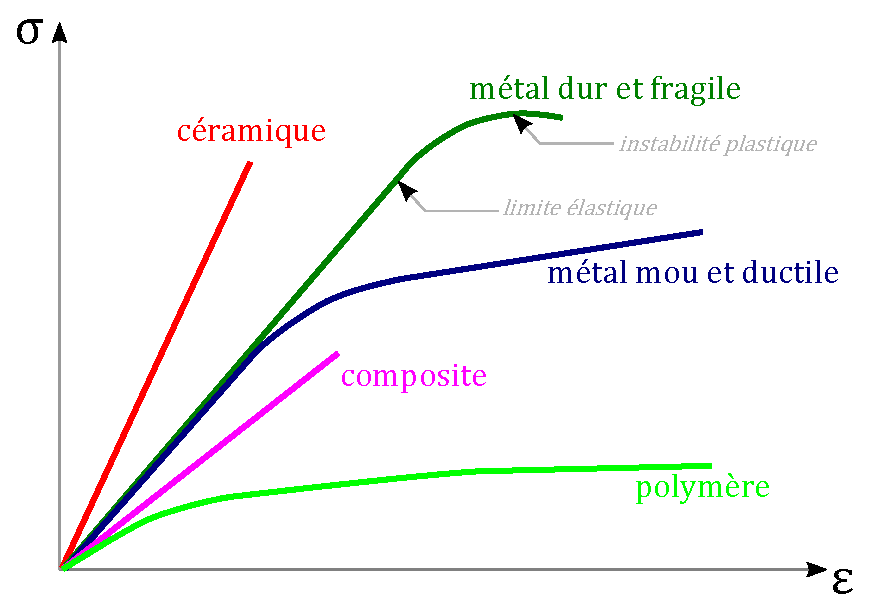
\includegraphics[height=5cm]{sig-eps.eps}}
  \caption{\label{Fig-sig-eps} Quelques lois types de comportement pour différents matériaux.}
\end{figure}

\medskip
Dans le cas de matériaux \textcolorblue{isotropes} (i.e. possédant les mêmes propriétés matérielles quelque soit l'orientation), les relations constitutives s'écrivent à l'aide des coefficients de Lamé~$\lambda$ et~$\mu$:\index{coefficients de Lamé}\index[aut]{Lame@Lamé (Gabriel), 1795-1870, Français}
%\footnote{%
%\begin{tabular}{ccc}
%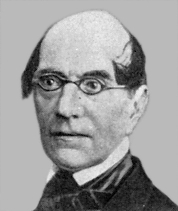
\includegraphics[height=32mm]{Lame}&
%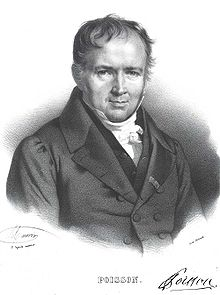
\includegraphics[height=32mm]{Poisson}&
%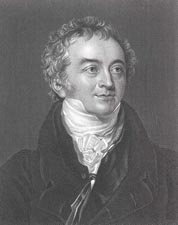
\includegraphics[height=32mm]{YoungT}\\
%Gabriel Lamé (Gabriel)&
%Siméon Denis Poisson&
%Thomas Young\\
%1795-1870&
%1781-1840&
% 1773-1829\\
%\end{tabular}}
\begin{equation}\sigma = 2\mu\varepsilon+\lambda \trace(\varepsilon)I\end{equation}
i.e.~$\sigma_{ij}=2\mu\varepsilon_{ij}+\lambda\varepsilon_{kk}\delta_{ij}$.
On rappelle également que:
\begin{equation}\lambda=\dfrac{E}{2(1+\nu)} \quad \text{ et } \quad \mu=\dfrac{E\nu}{(1-2\nu)(1+\nu)}
\end{equation}
avec~$E$ le module d'Young et~$\nu$ le coefficient de Poisson, que l'on exprime, inversement:\index[aut]{Young (Thomas), 1773-1829, Anglais}\index{coefficients de Poisson}\index[aut]{Poisson (Siméon Denis), 1781-1840, Français}\index{module d'Young}
\begin{equation}
E=\dfrac{\mu(3\lambda+2\mu)}{\lambda+\mu} \quad\text{ et }\quad
\nu=\dfrac{\lambda}{2(\lambda+\mu)}
\end{equation}
Pour assurer que la matrice~$H$ est définie positive, il faut que~$0<\nu<0,5$.

\medskip
Le cas~$\nu=0,5$ correspond au cas d'un matériau \textcolorred{incompressible}, comme par exemple le caoutchouc.\index{loi de comportement!incompressible} Nous verrons que selon les formulations il est plus ou moins aisé de prendre en compte ces matériaux. De plus, la littérature ne manque pas sur le sujet.

\medskip
\begin{wrapfigure}{l}{60mm}
  \centering
  \subfloat[Matériau compressible]{\includegraphics[width=28mm]{mtx_poisson.eps}} \hfill
  \subfloat[Matériau incompressible]{\includegraphics[width=28mm]{mtx_incompressible}}
  \caption{Déformation et coefficient de Poisson}
\end{wrapfigure}
\colorgreen
La signification physique du coefficent de Poisson est simple: $2\nu$ traduit le pourcentage de déformation dans le sens transverse à l'effort. En restant dans le cas plan, quand on fait subit à une pièce un effort de compression telle qu'elle subit une déformation (de compression) de 1, alors elle s'élargit de~$2\nu$ dans la direction transverse ($\nu$ de chaque côté par symétrie).

Ainsi, il devient évident qu'un matériau incompressible\index{loi de comportement!incompressible} est caractérisé par~$2\nu=1$, i.e. lorsqu'il perd un volume~$1$ selon une direction, il reprend un volume~$1$ dans la direction transverse: en d'autres termes, il ne varie pas de volume, il est donc incompressible [ce qui ne veut pas dire «incomprimable»!].

\medskip
Attention, cette signification physique du coefficient de Poisson n'est exacte que dans le cas de matériaux non seulement isotropes mais pleins. Pour un assemblage de matériaux ou de géométries, cette relation est mise en défaut, tout comme pour des matériaux orthotropes.

\medskip
\begin{wrapfigure}{r}{60mm}
  \centering
  \includegraphics[width=55mm]{mtx_auxetique.eps}
  \caption{Matériau auxétique}\label{fig-aux}
\end{wrapfigure}
Si l'on considère un matériau constitué d'alvéoles (de type hexagonal), mais dont les pointes sont rentrantes et non sortantes (figure~\ref{fig-aux}), alors le coefficient de Poisson macroscopique de ce matériau est négatif: quand on le comprime, il ne gonfle pas mais rétrécit.

On parle alors d'un matériau auxétique.\index{loi de comportement!auxétique}

On voit bien que dans un tel cas, la différence de comportement n'est due qu'à l'effet structurel, qu'à l'assemblage. Le matériau constituant les alvéoles lui, peut (et est) tout à fait conventionnel: on trouve ce genre de structures en carton, en aluminium et en acier, qui sont tous des matériaux homogènes isotropes.


\medskip
\begin{wrapfigure}{l}{70mm}
  \centering
  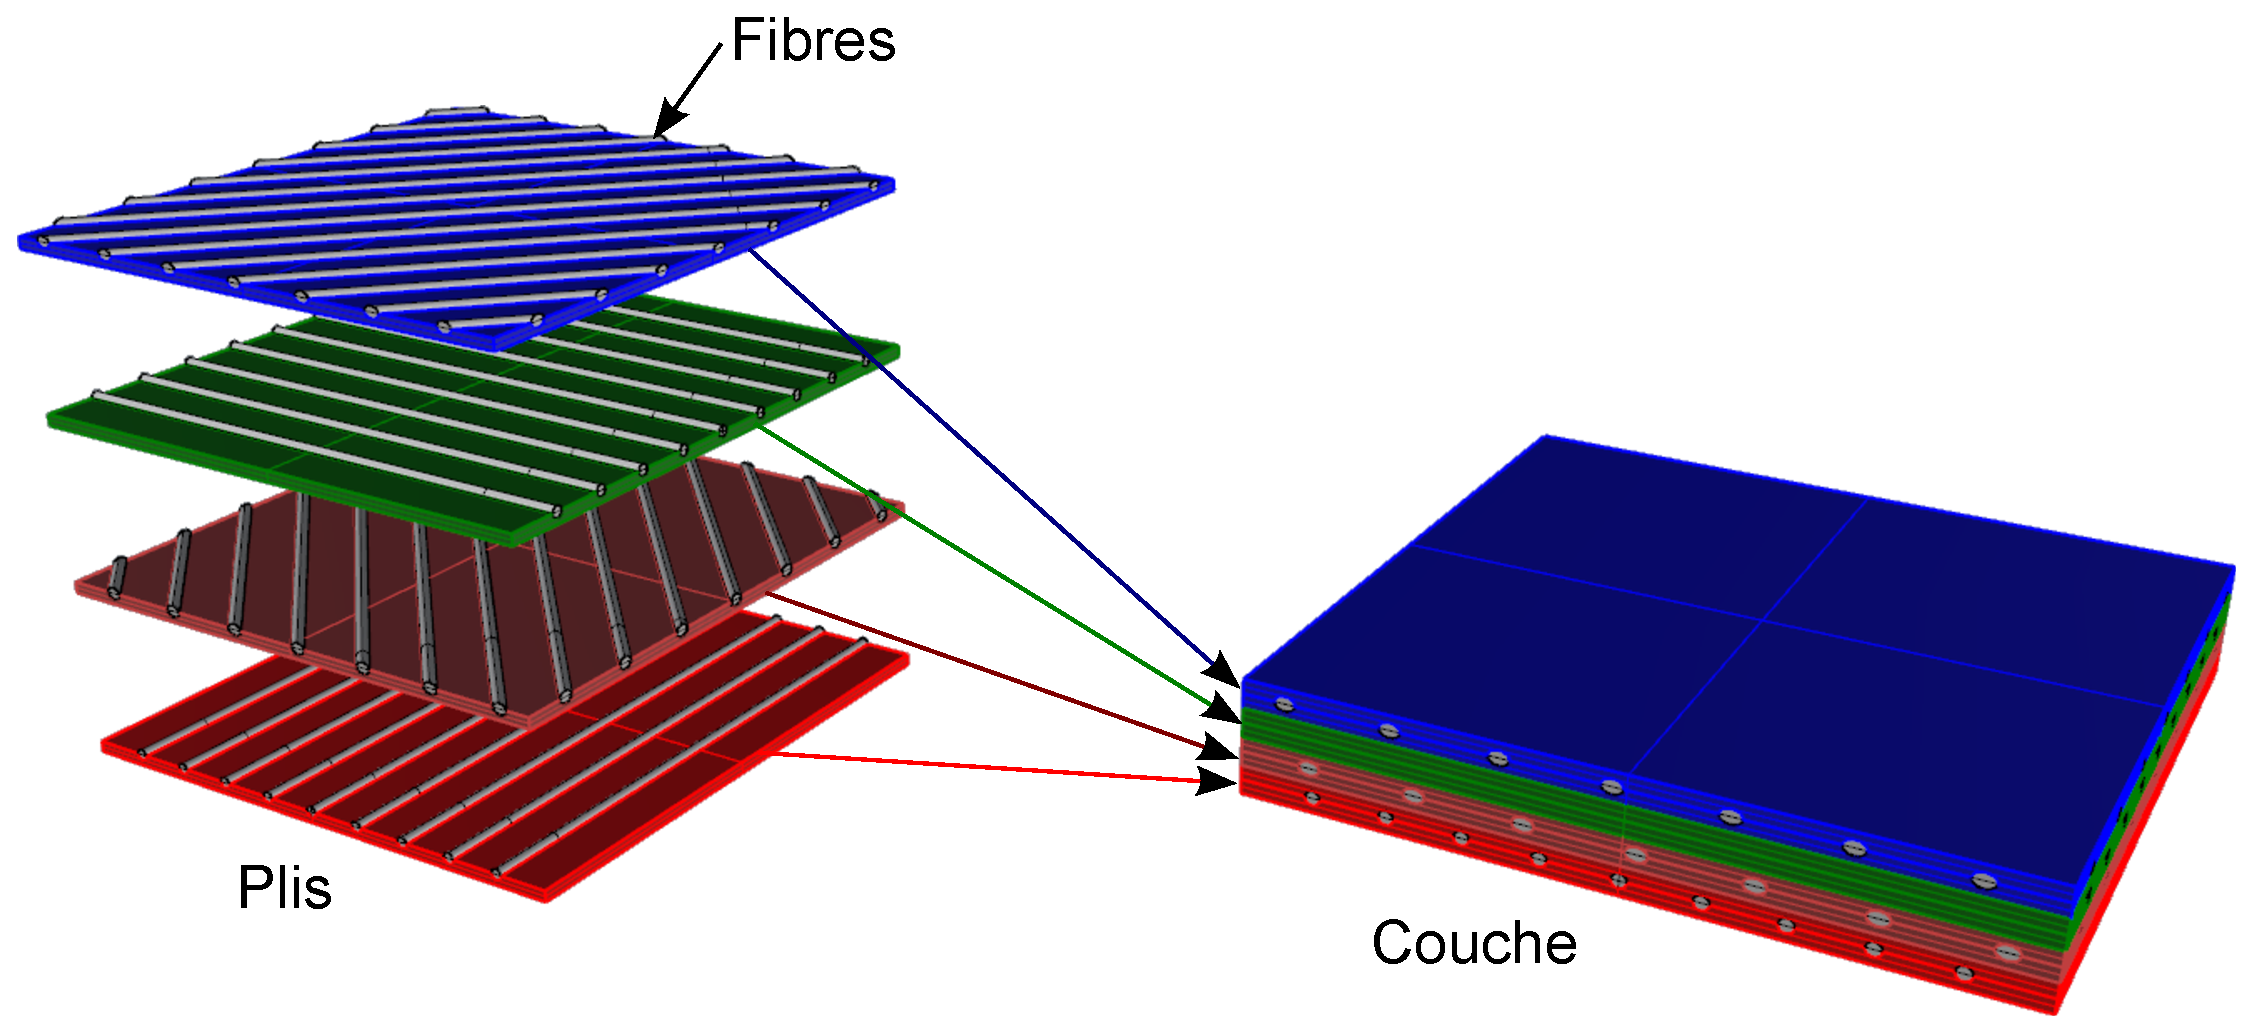
\includegraphics[width=70mm]{mtx-comp3.eps}
  \caption{Matériau composite}\label{fig-comp}
\end{wrapfigure}
Par exemple, la rigidité globale d'un assemblage de couches de composites renforcés de fibres, comme montré à la figure~\ref{fig-comp} peut conduire, selon les orientations des plis, à des valeurs du coefficient de Poisson très variables, d'autant plus que celles-ci sont fonctions du repère dans lequel elles sont données (repère global, repère des fibres...)

Un stratifié unidirectionnel T300 fibre de carbone/résine époxyde 934 a un coefficient de Poisson de seulement $\nu_{12}=0,04$.

Un stratifié unidirectionnel T300 fibre de carbone/résine N5208 a un coefficient de Poisson de $\nu_{12}=0,3$ dans le sens des fibres, mais de $\nu_{12}=-0,77$ à 45\degres.

En utilisant du verre ($E=69$~GPa, $\nu=0,25$) et de la résine époxyde ($E=3,5$~GPa, $\nu=0,4$), on peut réaliser un stratifié unidirectionnel verre-époxyde ayant pour propriétés $E_{ll}=45$~GPa, $E_{tt}=12$~GPa, $G_{lt}=4,5$~GPa, $\nu_{lt}=0,3$ pour une fraction volumique de verre de 60\%, et un stratifié [0/90] ayant pour propriétés $E_x=E_y=20$~GPa, $G_{xy}=2.85$~GPa et $\nu_{xy}=0.13$ pour une fraction volumique de verre de 50\%.

\colorblack

\medskip
Notons également que si~$\mu\ne0$ et~$3\lambda+2\mu\ne0$, alors on peut inverser la
relation contrainte/dé\-pla\-ce\-ment:
\begin{equation}
\varepsilon_{ij}=\dfrac1{2\mu}\left(\sigma_{ij}-\dfrac\lambda{3\lambda+2\mu}\trace(\sigma)\delta_{ij}\right)
\end{equation}

\medskip
Nous reviendrons plus tard sur ces aspects non linéaires au chapitre~\ref{Ch-NL}.


\medskip
\section{Équations de l'acoustique}\label{Sec-EqAcou}\index{ED-EDP!de l'acoustique}
L'acoustique, de manière la plus générale, a pour objet l'étude des sons et des ondes mécaniques.  Elle fait appel aux phénomènes ondulatoires et à la mécanique vibratoire.

\textcolorblue{C'est là tout «le problème» de la vibro-acoustique: elle met en jeu des échelles d'énergies très différentes.}
Considérons l'étude vibro-acoustique d'un véhicule. Alors, on doit aussi bien prendre en compte les effets mécaniques ayant une forte énergie (la rotation du moteur fait bouger tout le véhicule), que des effets ayant une énergie comparativement très faible: la composante aérienne du bruit. \textcolorgreen{Dans le premier cas, vous êtes face à quelque chose capable de faire «sauter» une voiture sur place, alors que dans le second vous êtes face au déplacement d'une feuille de papier lorsque vous criez devant elle!}

\medskip
Il est clair qu'il sera nécessaire d'étudier chaque aspect:
\begin{itemize}
\item \textcolorblue{solidien/solidien:} il s'agit d'une étude mécanique «classique», bien que l'on se trouve dans le cas d'une sollicitation qui dépend du temps. Celle-ci est d'ailleurs généralement périodique, d'où l'utilisation d'outils appropriés (en fréquence). On est dans le cas de propagation solidienne d'onde;
  \item \textcolorblue{aérien/aérien:} il s'agit de la propagation d'une onde acoustique de sa source jusqu'au récepteur. On est en présence d'un modèle purement de propagation
	d'onde;
  \item \textcolorblue{solidien/aérien:} il s'agit du cas du rayonnement. Une vibration mécanique fait vibrer un élément qui se met à émettre une onde dans l'air;
  \item \textcolorblue{aérien/solidien:} dans le cas de sources acoustiques très puissantes, l'onde acoustique se propageant dans l'air peut arriver à déformer et à faire vibrer une surface physique (par exemple un tablier de voiture).
\end{itemize}
Les deux derniers cas sont typiquement des cas dits de couplage fluide/structure.

\medskip
D'un point de vue de la formulation de ce problème sous forme d'équation aux dérivées partielles, tout à été dit précédemment. Nous verrons plus loin comment prendre en compte tous ces aspects de manière plus appliquée.

\medskip
\section{Multiplicateurs de Lagrange}\index{multiplicateurs de Lagrange}\index[aut]{Lagrange (Joseph Louis, comte de -), 1736-1813, Italien}

Les multiplicateurs de Lagrange ont une grande utilité, car leurs applications sont
vraiment très larges. \textcolorgreen{Pour rester très général, on va dire qu'ils permettent de «faire des liens» entre des grandeurs.} Nous allons expliquer cela sur quelques exemples.

\medskip
Si l'on reprend les équations de l'élasticité, on peut les réécrire en fonction uniquement des déplacements. L'avantage est que l'on dispose qu'un problème qui ne dépend que d'un unique champ inconnu, pour lequel les conditions aux limites correspondent à des choses très physiques: les déplacements imposés (appui simple, encastrement, contact).

Lorsque l'on résout un problème avec uniquement le champ de déplacements, alors évidemment, on obtient le champ de déplacements, mais uniquement lui! Alors comment remonter aux autres grandeurs? En utilisant les relations existantes... mais: entre déplacement et déformation, on a une dérivation, qui peut faire perdre en qualité d'approximation, d'autant plus lorsque l'on néglige les termes du second ordre.
Ensuite on se sert des relations entre déformation et contraintes, mais encore faut-il être capable de mesurer ces grandeurs... et même si l'on sait le faire, que se passe-t-il à l'interface entre deux matériaux distincts, comme par exemple entre l'une des peaux et l'âme d'un matériau sandwich? (sur le sujet, abordé en plusieurs fois dans ce document, voir synthèse au paragraphe~\ref{Sec-interf})

\medskip
Le cas du calcul des contraintes à l'interface entre deux matériaux est un exemple typique d'application des multiplicateurs de Lagrange. Si l'on considère chacun des deux matériaux comme indépendant, alors au sein de chaque matériau, les relations fonctionnent.
Si l'on impose maintenant la \textcolorblue{continuité des déplacements à l'interface} entre les deux matériaux (en écrivant que~$\lambda$ (qui représente les multiplicateurs de Lagrange) multiplié par la différence entre les déplacements de part et d'autre de l'interface est nul: analogie immédiate avec les résidus pondérés -- voir chapitre suivant), alors on s'aperçoit (ce sera détaillé dans le chapitre sur les formulations variationnelles) que les multiplicateurs de Lagrange s'interprètent comme les composantes des contraintes qui doivent être continues à l'interface (on parle de trace... comme défini au chapitre sur les espaces de Sobolev).

\medskip
Si maintenant l'un des domaines est l'air et l'autre la structure considérée, alors on se doute que les multiplicateurs de Lagrange peuvent servir à «faire le lien» entre ces deux domaines, à les \textcolorblue{coupler} en écrivant une équation liant la pression dans le fluide aux efforts de surface sur la structure par exemple... On voit comment on peut résoudre les problèmes évoqués dans le court paragraphe sur l'acoustique.

\medskip
Mais les multiplicateurs de Lagrange peuvent également être utilisés directement afin d'améliorer les méthodes numériques: ils permettent par exemple de «passer» les informations entre des maillages incompatibles, permettant par exemple de circonscrire une zone de maillage raffiné (avec raffinement automatique en plus si l'on veut) et une zone de maillage plus léger...

Une illustration de leur utilisation pour imposer des conditions aux limites en déplacement est donnée en~\ref{Ch-DispLag}.

\medskip
\textcolorgreen{%
Les multiplicateurs de Lagrange peuvent être introduits partout où l'on veut créer un lien entre des grandeurs, et cela sans se soucier de leur signification physique. Toutefois, dans de nombreux cas, il se trouve que ces multiplicateurs représentent certaines grandeurs, permettant une analogie entre différentes formulation d'un même problème.}



